\documentclass{ieeetj}
\usepackage{cite}
\usepackage{amsmath,amssymb,amsfonts,amsthm}
\usepackage{graphicx,color}
\usepackage{textcomp}
\usepackage{xcolor}
\usepackage{hyperref}
\hypersetup{hidelinks=true}
\usepackage{booktabs}
\usepackage{multirow}
\usepackage{float}

% Fix font substitutions for missing phv and pcr metrics in TeX Live Basic
\DeclareFontFamily{OT1}{phv}{}
\DeclareFontShape{OT1}{phv}{m}{n}{<-> ssub * cmss/m/n}{}
\DeclareFontShape{OT1}{phv}{b}{n}{<-> ssub * cmss/bx/n}{}
\DeclareFontShape{OT1}{phv}{m}{it}{<-> ssub * cmss/m/it}{}
\DeclareFontShape{OT1}{phv}{b}{it}{<-> ssub * cmss/bx/it}{}
\DeclareFontShape{OT1}{phv}{m}{sl}{<-> ssub * cmss/m/sl}{}
\DeclareFontShape{OT1}{phv}{b}{sl}{<-> ssub * cmss/bx/sl}{}

\DeclareFontFamily{OT1}{pcr}{}
\DeclareFontShape{OT1}{pcr}{m}{n}{<-> ssub * cmtt/m/n}{}
\DeclareFontShape{OT1}{pcr}{b}{n}{<-> ssub * cmtt/m/n}{}
\DeclareFontShape{OT1}{pcr}{m}{it}{<-> ssub * cmtt/m/n}{}
\DeclareFontShape{OT1}{pcr}{b}{it}{<-> ssub * cmtt/m/n}{}


\providecommand{\FloatBarrier}{}

\setlength{\textfloatsep}{3pt plus 1pt minus 1pt}
\setlength{\floatsep}{3pt plus 1pt minus 1pt}
\setlength{\intextsep}{3pt plus 1pt minus 1pt}

\def\BibTeX{{\rm B\kern-.05em{\sc i\kern-.025em b}\kern-.08em
    T\kern-.1667em\lower.7ex\hbox{E}\kern-.125emX}}
\AtBeginDocument{\definecolor{tmlcncolor}{cmyk}{0.93,0.59,0.15,0.02}\definecolor{NavyBlue}{RGB}{0,86,125}}

\def\OJlogo{\vspace{-4pt}IEEE Open Journal of the Computer Society}
\def\seclogo{\vspace{10pt}IEEE Open Journal of the Computer Society}

\def\authorrefmark#1{\ensuremath{^{\textbf{#1}}}}

\newtheorem{theorem}{Theorem}
\newtheorem{remark}{Remark}

\begin{document}
\jvol{14}
\jnum{01}
\pubyear{2026}


\markboth{Cost-Sensitive Conformal Prediction for Imbalanced Decisions}{Singh \textit{et al.}}

\title{Cost-Sensitive Conformal Prediction and Human-in-the-Loop Abstention for Imbalanced High-Stakes Decision Support: A Multi-Domain Benchmark}

\author{Manpreet Singh\authorrefmark{1}, Senior Member, IEEE, Akshatha Srikantha\authorrefmark{2}, Deepak Parashar\authorrefmark{3}, and Rahul Joshi\authorrefmark{4}}
\affil{Boston University, Boston, MA 02215 USA}
\affil{University of California, Irvine, Irvine, CA 92697 USA}
\affil{Manipal Institute of Technology, Manipal Academy of Higher Education, Manipal 576104, India}
\affil{Symbiosis Institute of Technology, Pune,  Symbiosis International (Deemed University), Pune, India}
\corresp{Corresponding author: Deepak Parashar (email: deepak.parashar@manipal.edu).}

\begin{abstract}
High-stakes decision systems in credit scoring, fraud detection, healthcare, and industrial safety require uncertainty quantification under severe class imbalance and asymmetric error costs. Standard marginal conformal prediction (CP) provides valid overall coverage, but under-covers rare classes (averaging 30.77\% minority-class coverage across 3,150 experimental fits in our multi-domain evaluation). Mondrian CP restores minority validity, achieving 92.12\% mean minority coverage (+61.35 percentage-point gain over marginal CP). We evaluate Mondrian prediction sets combined with cost-sensitive deferral across 15 imbalanced tabular datasets, 7 classifiers, 3 probability calibrators, and 10 random seeds. Under realistic human review costs ($C_{\mathrm{rev}}=0.50$) and human queue capacity constraints ($r_{\max}=10.00\%$), capacity-limited Mondrian deferral achieves a mean decision cost of 0.45 at an 8.50\% abstention rate, compared with Bayes point thresholding (0.34) and unconstrained cost-controlled deferral (0.37 cost, 67.03\% abstention). Negative break-even review thresholds ($C_{\mathrm{rev}}^* < 0$) arise on three datasets through two distinct mechanisms: sparse minority calibration samples inflating quantile variance, and heavy posterior overlap near the Bayes decision boundary on well-balanced but high-noise tasks. We quantify operational capacity limits, reviewer error rates ($\epsilon_{\mathrm{hum}}$), and dataset-specific break-even thresholds ($C_{\mathrm{rev}}^*$), establishing explicit boundary conditions where human deferral is economically viable.
\end{abstract}

\begin{IEEEkeywords}
Conformal prediction, Imbalanced classification, Cost-sensitive learning, Selective classification, Uncertainty quantification, Decision support systems.
\end{IEEEkeywords}

\maketitle

\section{Introduction}
\label{sec:intro}

\IEEEPARstart{M}{achine} learning models in knowledge-based decision support systems (credit scoring, fraud detection, healthcare, industrial safety) face asymmetric error costs: failing to detect rare positive events incurs penalties far exceeding false alarms \cite{he2009learning, herbei2006classification, bartlett2008classification}. Standard point predictors and raw confidence scores fail to provide reliable uncertainty estimates in high-stakes operations.

Conformal prediction (CP) offers distribution-free, finite-sample $1-\alpha$ coverage guarantees \cite{vovk2005algorithmic, angelopoulos2021gentle}. However, standard marginal CP guarantees validity only on average across the data distribution \cite{lei2018distribution}. Under severe class imbalance, marginal CP satisfies global targets by over-covering the majority class while minority-class coverage drops near zero (averaging 30.77\% across our benchmark). Class-conditional (Mondrian) CP resolves this by computing per-class non-conformity quantiles, enforcing $1-\alpha$ coverage independently per class \cite{vovk2005algorithmic, sadinle2019least, lofstrom2015bias, norinder2017applying}. While prior work confirmed coverage restoration on imbalanced data \cite{toccaceli2019combination}, how Mondrian sets interact with asymmetric error costs, human review overhead ($C_{\mathrm{rev}}$), and review queue limits ($r_{\max}$) remains unstudied.

To address this gap, we evaluate conformal decision deferral across 15 imbalanced tabular datasets, 7 classifiers, 3 calibration methods, and 10 random seeds (3,150 fits). Our primary contributions are:
\begin{enumerate}
    \item \textbf{Multi-Domain Benchmark}: Evaluation across 15 tabular datasets, 7 classifiers, and 3 calibration regimes confirming a 61.35 percentage-point minority coverage gain for Mondrian CP over marginal CP.
    \item \textbf{Selection-Split Calibration}: A split-conformal protocol decoupling miscoverage selection ($\alpha^*$) from final quantile estimation, with conditional class-wise validity guarantees.
    \item \textbf{Capacity-Constrained Cost Modeling \& Deployment Boundaries}: Formalization of capacity-constrained deferral under review costs ($C_{\mathrm{rev}}$) and queue limits ($r_{\max} = 10\%$), reviewer error rates ($\epsilon_{\mathrm{hum}}$), and deriving closed-form empirical break-even thresholds ($C_{\mathrm{rev}}^*$).
\end{enumerate}

\section{Related Work}
\label{sec:related_work}

\subsection{Conformal Prediction \& Distribution-Free Uncertainty Quantification}
Conformal prediction constructs valid finite-sample prediction sets \cite{vovk2005algorithmic, angelopoulos2021gentle, papadopoulos2002inductive}. Adaptive Prediction Sets (APS) and Regularized APS (RAPS) aggregate cumulative probabilities to trim set sizes \cite{romano2020classification, angelopoulos2021uncertainty, huang2024saps}. Standard marginal CP fails under class imbalance because global validity permits under-covering rare classes \cite{lei2018distribution}. Class-conditional (Mondrian) CP calculates per-class quantiles to restore class-specific validity \cite{vovk2005algorithmic, sadinle2019least, vovk2012conditional, lofstrom2015bias, norinder2017applying, toccaceli2019combination, bostrom2021mondrian}. Recent extensions address multi-class efficiency \cite{ding2023class, shi2024rc3p}, end-to-end training \cite{stutz2022learning}, non-stationary drift \cite{gibbs2021adaptive}, and risk control \cite{angelopoulos2024risk, bartlett2008classification}. None analyze monetary decision costs under capacity-constrained human review in decision support systems.

\subsection{Cost-Sensitive Learning \& Selective Deferral}
Cost-sensitive classification optimizes decisions under asymmetric penalties ($C_{\mathrm{FN}} \gg C_{\mathrm{FP}}$) \cite{elkan2001foundations, weiss2004mining, he2009learning}. When $C_{\mathrm{FN}} > C_{\mathrm{FP}}$, the Bayes-optimal rule threshold is $\tau^* = \frac{C_{\mathrm{FP}}}{C_{\mathrm{FN}} + C_{\mathrm{FP}}}$ \cite{elkan2001foundations}. Traditional methods rely on probability calibration (Platt scaling, isotonic regression) \cite{zadrozny2002transforming, guo2017calibration} but force hard single-label assignments without abstention.

Selective classification enables classifiers to abstain on uncertain predictions \cite{chow1970optimum, elyaniv2010foundations, geifman2017selective, cortes2016rejection, geifman2019selectivenet}. Learning to Defer (L2D) joint-trains rejection policies based on expert costs \cite{mozannar2020consistent, hemmer2021complementarity, charoenphakdee2021rejection}. In distribution-free settings, conformal risk control bounds set losses \cite{angelopoulos2024risk}, and set-valued prediction improves human-AI team performance \cite{straitouri2023improving, straitouri2024decision}. We bridge these domains by evaluating Mondrian conformal sets under explicit review costs ($C_{\mathrm{rev}}$), reviewer errors ($\epsilon_{\mathrm{hum}}$), and queue capacity limits ($r_{\max}$).

\section{Methodology \& Theoretical Framework}
\label{sec:methodology}

This section details the theoretical and operational framework of cost-sensitive conformal prediction for imbalanced classification in knowledge-based decision support systems.

\subsection{Problem Formulation \& Asymmetric Cost Matrix}
Consider a binary classification task where input features $X \in \mathcal{X} \subseteq \mathbb{R}^d$ map to a true class label $Y \in \mathcal{Y} = \{0, 1\}$. Label $Y=1$ denotes the rare, costly positive class (such as fraudulent transaction, medical disease, or equipment failure), while $Y=0$ denotes the majority negative class. Let $\pi_1 = P(Y=1) \in (0, 0.5)$ represent the prior prevalence of the minority class, indicating severe data imbalance ($\pi_1 \ll 0.5$).

We define an asymmetric decision cost matrix $\mathbf{C} \in \mathbb{R}_{\ge 0}^{2 \times 2}$, where $C_{ij}$ represents the cost incurred by predicting class $j \in \{0, 1\}$ when the true label is $i \in \{0, 1\}$:
\begin{equation}
\mathbf{C} = \begin{bmatrix} C_{00} & C_{01} \\ C_{10} & C_{11} \end{bmatrix} = \begin{bmatrix} 0 & C_{\mathrm{FP}} \\ C_{\mathrm{FN}} & 0 \end{bmatrix}
\end{equation}
Correct decisions carry zero cost ($C_{00} = C_{11} = 0$). False positive predictions incur penalty $C_{\mathrm{FP}}$, while false negative predictions incur penalty $C_{\mathrm{FN}}$. In high-stakes domains, failure to detect a positive case carries far greater risk than a false alarm, establishing $C_{\mathrm{FN}} \gg C_{\mathrm{FP}}$.

When automated predictions exhibit high ambiguity, the system can abstain from a single hard decision and defer the sample to a human expert. Deferring an instance incurs operational review cost $C_{\mathrm{rev}} > 0$. Reviewers are not infallible, so we attach a flat reviewer error rate $\epsilon_{\mathrm{hum}} \in [0,1)$ to deferred cases, giving expected per-instance deferral cost
\begin{equation}
\mathbb{E}[L_{\mathrm{defer}}] = C_{\mathrm{rev}} + \epsilon_{\mathrm{hum}} \cdot \bar{c}_{\mathrm{err}}, \quad \bar{c}_{\mathrm{err}} = (1-\bar{\pi}_1) C_{\mathrm{FP}} + \bar{\pi}_1 C_{\mathrm{FN}}
\end{equation}
where $\bar{c}_{\mathrm{err}}$ is the mean misclassification cost a mistaken reviewer incurs, evaluated at a pooled minority prevalence $\bar{\pi}_1 = 0.10$ across the benchmark. Human deferral remains economically rational only where expert error strictly beats automated model misclassification error ($\mathbb{E}[L_{\mathrm{defer}}] < \mathbb{E}[L_{\mathrm{point}}]$). We sweep $\epsilon_{\mathrm{hum}}$ post hoc over fixed Mondrian deferral masks; estimating an instance-dependent error rate would require per-instance reviewer labels and is left to future work.

\subsection{Marginal vs.\ Class-Conditional (Mondrian) Conformal Predictors}
Let $D_{\mathrm{cal}} = \{(X_i, Y_i)\}_{i=1}^{n_{\mathrm{cal}}}$ be an exchangeable calibration set independent of base classifier training data. For a candidate sample $X$ and label $y \in \{0, 1\}$, a machine learning model outputs estimated posterior class probability $\hat{P}(Y=y \mid X)$. Standard non-conformity uses predicted class error:
\begin{equation}
S(X, y) = 1 - \hat{P}(Y=y \mid X)
\end{equation}
A higher non-conformity score indicates lower model confidence for label $y$.

\subsubsection{Adaptive and Regularized Conformal Scores (APS and RAPS)}
To evaluate adaptive non-conformity baselines, we incorporate Adaptive Prediction Sets (APS) \cite{romano2020classification} and Regularized Adaptive Prediction Sets (RAPS) \cite{angelopoulos2021uncertainty}. Let $\hat{\pi}_{(1)}(X) \ge \hat{\pi}_{(2)}(X)$ denote sorted class probabilities, $k(y)$ denote the rank of candidate label $y$, and $U \sim \text{Unif}(0,1)$ denote a random tie-breaker.

The APS non-conformity score is defined as:
\begin{equation}
S_{\mathrm{APS}}(X, y) = \sum_{j=1}^{k(y)-1} \hat{\pi}_{(j)}(X) + U \cdot \hat{\pi}_{(k(y))}(X)
\end{equation}

RAPS incorporates a penalty parameter $\lambda \ge 0$ and size threshold $k_{\mathrm{reg}} \ge 1$ to trim set cardinalities; we set $k_{\mathrm{reg}} = 1$ throughout:
\begin{equation}
\begin{split}
S_{\mathrm{RAPS}}(X, y) = \sum_{j=1}^{k(y)} \hat{\pi}_{(j)}(X) &+ \lambda \max(0, k(y) - k_{\mathrm{reg}}) \\
&- U \cdot \hat{\pi}_{(k(y))}(X)
\end{split}
\end{equation}

\subsubsection{Marginal Conformal Prediction}
Standard marginal conformal prediction calculates a single non-conformity quantile $q_{\mathrm{marg}}$ across all calibration samples in $D_{\mathrm{cal}}$:
\begin{equation}
q_{\mathrm{marg}} = \text{Quantile}\!\left(\{S(X_i, Y_i)\}_{i=1}^{n_{\mathrm{cal}}}, \, \tfrac{\lceil (n_{\mathrm{cal}}+1)(1-\alpha) \rceil}{n_{\mathrm{cal}}}\right)
\end{equation}
For a test sample $X$, the marginal prediction set is constructed as:
\begin{equation}
\hat{C}_{\mathrm{marg}}(X) = \{y \in \{0, 1\} \mid S(X, y) \le q_{\mathrm{marg}}\}
\end{equation}
By distribution-free exchangeability, marginal CP guarantees global coverage:
\begin{equation}
P(Y \in \hat{C}_{\mathrm{marg}}(X)) \ge 1 - \alpha
\end{equation}
Under severe class imbalance ($\pi_1 \ll 0.5$), the marginal score distribution is dominated by majority-class samples ($Y=0$). As a result, $q_{\mathrm{marg}}$ settles near the majority-class quantile, allowing global coverage to hold while minority-class coverage ($Y=1$) drops near zero \cite{vovk2012conditional, ding2023class}.

\subsubsection{Class-Conditional (Mondrian) Conformal Prediction}
Mondrian conformal prediction restores coverage for rare classes by splitting $D_{\mathrm{cal}}$ into class-specific subsets $D_{\mathrm{cal}}^{(0)} = \{(X_i, Y_i) \in D_{\mathrm{cal}} \mid Y_i = 0\}$ of size $n_0$ and $D_{\mathrm{cal}}^{(1)} = \{(X_i, Y_i) \in D_{\mathrm{cal}} \mid Y_i = 1\}$ of size $n_1$. Independent quantiles $q_0$ and $q_1$ are computed for each class label:
\begin{equation}
\begin{split}
q_y = \text{Quantile}\!\left(\{S(X_i, Y_i)\}_{i \in D_{\mathrm{cal}}^{(y)}}, \, \tfrac{\lceil (n_y+1)(1-\alpha) \rceil}{n_y}\right), \\
y \in \{0, 1\}
\end{split}
\label{eq:mondrian_quantile}
\end{equation}
Under standard finite-sample discrete empirical quantile definitions, if class sample size $n_y$ is small enough that $\lceil (n_y+1)(1-\alpha) \rceil \ge n_y$ (at $\alpha=0.10$ this holds whenever $n_y \le 18$), the quantile index saturates and $q_y = \max_{i \in D_{\mathrm{cal}}^{(y)}} S(X_i, Y_i)$. Prediction sets then grow, but the attainable class-conditional coverage is capped at $n_y/(n_y+1)$, which lies \emph{below} the nominal $1-\alpha$. In our benchmark this regime affects four datasets: \texttt{oil\_spill} ($n_{1,\mathrm{cal}}=4$, cap $80.0\%$), \texttt{pc1} ($8$, $88.9\%$), \texttt{ozone\_level\_8hr} ($16$, $94.1\%$) and \texttt{seismic\_bumps} ($17$, $94.4\%$); on the first two the $90\%$ target is not attainable.

The Mondrian prediction set is formed by evaluating each candidate label against its class-specific quantile threshold:
\begin{equation}
\hat{C}_{\mathrm{Mondrian}}(X) = \{y \in \{0, 1\} \mid S(X, y) \le q_y\}
\label{eq:mondrian_set}
\end{equation}
For standard probability non-conformity $S(X,y) = 1 - \hat{P}(Y=y \mid X)$, candidate inclusions $S(X,1) \le q_1$ and $S(X,0) \le q_0$ map directly to an explicit decision probability interval for candidate label $y=1$:
\begin{equation}
\hat{P}(Y=1 \mid X) \in [1 - q_0, \, q_1]
\end{equation}
Specifically, $y=1 \in \hat{C}_{\mathrm{Mondrian}}(X)$ if and only if $\hat{P}(Y=1 \mid X) \ge 1 - q_1$, while $y=0 \in \hat{C}_{\mathrm{Mondrian}}(X)$ if and only if $\hat{P}(Y=1 \mid X) \le q_0$. When $1 - q_1 \le q_0$ (i.e., $q_0 + q_1 \ge 1$), posterior ambiguity produces multi-label set $\{0, 1\}$; when $q_0 + q_1 < 1$, non-overlapping thresholds can yield empty prediction set $\emptyset$.

This construction guarantees finite-sample class-conditional validity for both classes independently \cite{vovk2012conditional}:
\begin{equation}
P(Y \in \hat{C}_{\mathrm{Mondrian}}(X) \mid Y = y) \ge 1 - \alpha, \quad \forall y \in \{0, 1\}
\end{equation}

\subsection{Cost-Controlled Abstention Mechanism}\label{subsec:costctrl}
\textbf{Cost-Controlled Mondrian.} Standard Mondrian prediction sets construct non-conformity quantiles $(q_0, q_1)$ to satisfy class coverage target $1-\alpha$, remaining cost-agnostic during set formation. Operational cost sensitivity is realized at the decision level by selecting operating miscoverage level $\alpha^\star$ on a separate selection split $D_{\mathrm{sel}}$. We use the candidate grid $\mathcal{A}=\{0.01,0.03,\ldots,0.43,0.45\}$, consisting of 23 equally spaced values between 0.01 and 0.45. For each candidate, we construct class-conditional sets on the selection split, evaluate expected loss $\mathbb{E}[L]$ under $(C_{\mathrm{FP}}, C_{\mathrm{FN}}, C_{\mathrm{rev}})$, and choose $\alpha^\star = \arg\min_{\alpha \in \mathcal{A}} \widehat{\mathbb{E}}[L]$ among candidates whose selection-split minority coverage attains the target, $\widehat{P}_{D_{\mathrm{sel}}}(Y \in \hat{C}_\alpha(X) \mid Y=1) \ge 1-\alpha$; if none attains it we fall back to the most conservative grid point, $\alpha^\star = 0.01$.

When operational review capacity is constrained by a maximum human queue budget $r_{\max} \in (0,1)$, the benchmark enforces the budget with a post-hoc admission rule rather than by constrained selection of $\alpha^\star$: deferred instances are returned to automated decision in decreasing order of model confidence $\max_y \hat{P}(Y=y \mid X)$ until the deferral count falls below $\lfloor r_{\max} \cdot n \rfloor$. We report this variant as Capacity-Limited Mondrian.
\begin{remark}[Finite-Sample Queue Capacity Bound]
Because the admission rule is applied to the evaluation stream itself, the reported abstention rate is exact by construction rather than an out-of-sample estimate, and no safety margin is needed ($\epsilon = 0$). A deployment that instead selected $\alpha^\star$ on $D_{\mathrm{sel}}$ subject to $\hat{P}_{D_{\mathrm{sel}}}(|\hat{C}_\alpha(X)| \neq 1) \le r_{\max} - \epsilon$ would require one: Hoeffding/Clopper--Pearson bounds give $P(|\hat{C}_{\alpha^\star}(X)| \neq 1) \le \hat{P}_{D_{\mathrm{sel}}}(|\hat{C}_{\alpha^\star}(X)| \neq 1) + \sqrt{\ln(1/\delta)/(2 n_{\mathrm{sel}})}$ with probability at least $1-\delta$, so $\epsilon = \sqrt{\ln(1/\delta)/(2 n_{\mathrm{sel}})}$ yields PAC queue capacity control at level $1-\delta$.
\end{remark}

\subsubsection{Post-Selection Mondrian Coverage}
Selecting miscoverage level $\alpha^\star$ over grid $\mathcal{A}$ uses data separate from final conformal calibration. After model fitting and probability calibration, the held-out calibration pool is split into selection split $D_{\mathrm{sel}}$ and final calibration split $D_{\mathrm{cal}}$, each containing 50.00\% of that pool with stratified class proportions. The candidate level is chosen using only $D_{\mathrm{sel}}$. The tuned predictor is then fit once, using only $D_{\mathrm{cal}}$ to compute $(q_0(\alpha^\star),q_1(\alpha^\star))$. The test split is used in neither operation. Conditional on $D_{\mathrm{sel}}$, $\alpha^\star$ is fixed before final class-specific quantiles are computed.

\begin{theorem}[Conditional Mondrian Validity]
Assume calibration and test examples $\{(X_i, Y_i)\}_{i=1}^{n_{\mathrm{cal}}} \cup \{(X_{n+1}, Y_{n+1})\}$ are exchangeable within each class label $y \in \{0, 1\}$, selection split $D_{\mathrm{sel}}$ is independent of final calibration split $D_{\mathrm{cal}}$, and each class contains at least one observation in $D_{\mathrm{cal}}$ ($n_y \ge 1$). Conditional on $D_{\mathrm{sel}}$, the selected miscoverage target $\alpha^\star$ is fixed before quantiles $(q_0(\alpha^\star), q_1(\alpha^\star))$ are computed on $D_{\mathrm{cal}}$. For a future exchangeable test instance $(X_{n+1}, Y_{n+1})$, the split Mondrian prediction set $\hat{C}_{\alpha^\star}(X_{n+1})$ constructed from $D_{\mathrm{cal}}$ satisfies class-conditional coverage (see Appendix~B for formal proof):
\begin{equation}
P(Y_{n+1} \in \hat{C}_{\alpha^\star}(X_{n+1}) \mid Y_{n+1} = y) \ge 1 - \alpha^\star, \quad \forall y \in \{0, 1\}
\end{equation}
subject to the finite-sample quantile convention in \eqref{eq:mondrian_quantile} and to $\lceil (n_y+1)(1-\alpha^\star) \rceil \le n_y$; where that condition fails the guarantee holds only at the reduced level $n_y/(n_y+1)$.
\end{theorem}

Prediction set outputs $\hat{C}(X) \subseteq \{0, 1\}$ yield four possible set configurations: singletons ($\{0\}$ or $\{1\}$), multi-label ambiguities ($\{0, 1\}$), or empty sets ($\emptyset$). We define an operational decision rule $\hat{Y}_{\mathrm{action}}(X)$ that maps prediction set outputs to automated decisions or human deferral:
\begin{equation}
\hat{Y}_{\mathrm{action}}(X) = \begin{cases} 
0, & \text{if } \hat{C}(X) = \{0\} \\
1, & \text{if } \hat{C}(X) = \{1\} \\
\text{DEFER}, & \text{if } |\hat{C}(X)| \neq 1
\end{cases}
\end{equation}

An empty prediction set occurs when a sample exhibits high non-conformity across all class distributions ($S(X,y) > q_y$ for both $y \in \{0,1\}$), which may indicate atypical or out-of-distribution feature patterns. Treating both multi-label ambiguities and empty set outputs as abstention triggers ensures that any non-singleton prediction ($|\hat{C}(X)| \neq 1$) is safely routed to human expert review.

When $|\hat{C}(X)| = 1$, the automated decision is executed. If the single label matches the true class $Y$, decision cost is zero. If the automated prediction is incorrect, cost $C_{\mathrm{FP}}$ or $C_{\mathrm{FN}}$ is incurred. When $|\hat{C}(X)| \neq 1$, the system abstains and defers the case to human review. Under expert oracle assumptions ($\epsilon_{\mathrm{hum}} = 0$), the per-instance decision loss $L(Y, \hat{C}(X))$ is formalized as:
\begin{equation}
L(Y, \hat{C}(X)) = \begin{cases}
0, & \text{if } \hat{C}(X) = \{Y\} \\
C_{\mathrm{FP}}, & \text{if } \hat{C}(X) = \{1\} \text{ and } Y = 0 \\
C_{\mathrm{FN}}, & \text{if } \hat{C}(X) = \{0\} \text{ and } Y = 1 \\
C_{\mathrm{rev}}, & \text{if } |\hat{C}(X)| \neq 1
\end{cases}
\end{equation}

\subsection{Theoretical Break-Even Derivation}
We derive the critical human review cost threshold $C_{\mathrm{rev}}^*$ below which a fixed Mondrian deferral policy achieves lower total expected decision cost than the cost-tuned point-threshold baseline used in the benchmark.

Let $\tau^* = \frac{C_{\mathrm{FP}}}{C_{\mathrm{FN}} + C_{\mathrm{FP}}}$ denote the cost threshold applied to estimated probabilities. A point predictor using threshold $\tau^*$ yields false positive rate $\mathrm{FPR}_{\tau^*}$ and false negative rate $\mathrm{FNR}_{\tau^*}$. The expected per-instance cost of point classification $\mathbb{E}[L_{\text{point}}]$ is:
\begin{equation}
\mathbb{E}[L_{\text{point}}] = (1-\pi_1) \cdot C_{\mathrm{FP}} \cdot \mathrm{FPR}_{\tau^*} + \pi_1 \cdot C_{\mathrm{FN}} \cdot \mathrm{FNR}_{\tau^*}
\end{equation}

For the cost-controlled Mondrian conformal predictor, let $r_{\mathrm{abs}} = P(|\hat{C}(X)| \neq 1)$ denote the total abstention rate. Let $\mathrm{FPR}_{\mathrm{conf}} = P(\hat{C}(X)=\{1\} \mid Y=0)$ denote the automated false positive rate, and let $\mathrm{FNR}_{\mathrm{conf}} = P(\hat{C}(X)=\{0\} \mid Y=1)$ denote the automated false negative rate on singleton predictions. The expected per-instance cost $\mathbb{E}[L_{\mathrm{conf}}]$ is:
\begin{equation}
\begin{split}
\mathbb{E}[L_{\mathrm{conf}}] = (1-\pi_1) C_{\mathrm{FP}} \mathrm{FPR}_{\mathrm{conf}} &+ \pi_1 C_{\mathrm{FN}} \mathrm{FNR}_{\mathrm{conf}} \\
&+ r_{\mathrm{abs}} C_{\mathrm{rev}}
\end{split}
\end{equation}

Setting $\mathbb{E}[L_{\mathrm{conf}}] < \mathbb{E}[L_{\text{point}}]$ and solving for $C_{\mathrm{rev}}$ yields the break-even human review threshold $C_{\mathrm{rev}}^*$:
\begin{equation}
C_{\mathrm{rev}}^* = \frac{\mathbb{E}[L_{\mathrm{point}}] - \mathbb{E}[L_{\mathrm{conf}}]\big|_{C_{\mathrm{rev}}=0}}{r_{\mathrm{abs}}}
\end{equation}
Under the stated cost matrix and exchangeability conditions, the fixed-policy estimate is lower than the cost-tuned point baseline when $C_{\mathrm{rev}} < C_{\mathrm{rev}}^*$. This threshold is an empirical comparison based on repeated benchmark configurations. Specifically, $C_{\mathrm{rev}}^*$ represents an ideal upper-bound threshold assuming zero queue congestion ($W=0$, static service rate under capacity $\rho < 1$). Under operational queue congestion ($\rho \to 1$), request arrival rate $\lambda_{\mathrm{rev}} = \lambda \cdot r_{\mathrm{abs}}$ induces non-zero queue wait times $W > 0$, adding a dynamic queue delay penalty $\mathbb{E}[C_{\mathrm{delay}}(W)]$ (Section~\ref{sec:architecture}). Active queuing shifts the economic viability boundary downward to $C_{\mathrm{rev}}^* - \mathbb{E}[C_{\mathrm{delay}}(W)]/r_{\mathrm{abs}}$, establishing that static evaluation overestimates human deferral cost-effectiveness under heavy workload arrival rates.

\section{Experimental Setup}
\label{sec:exp_setup}

This section outlines the benchmark datasets, machine learning models, baseline methods, and statistical metrics used to evaluate cost-sensitive conformal prediction.

\subsection{Benchmark Datasets \& Taxonomy}
We evaluate the framework across 15 public tabular datasets from OpenML, covering credit scoring, financial fraud, medical diagnosis, industrial safety, remote sensing, and environmental monitoring. Table~\ref{tab:dataset_taxonomy} summarizes dataset characteristics, sample counts ($n$), feature counts ($d$), minority class percentages ($\pi_1$), and imbalance ratios.

\begin{table*}[!htbp]
\caption{Taxonomy of 15 OpenML tabular benchmark datasets.}
\label{tab:dataset_taxonomy}
\centering
\small
\renewcommand{\arraystretch}{0.88}
\resizebox{0.92\textwidth}{!}{%
\begin{tabular}{llrrrcc}
\hline
Dataset Name & Domain & Samples ($n$) & Features ($d$) & Minority Class (\%) & Imbalance Ratio & Minority $n_{1,\mathrm{cal}}$ \\
\hline
uci\_default & Finance & 30,000 & 23 & 22.12\% & 3.52 : 1 & 664 \\
bank\_marketing & Marketing & 45,211 & 16 & 11.70\% & 7.55 : 1 & 529 \\
adult & Demographics & 48,842 & 14 & 23.93\% & 3.18 : 1 & 1,169 \\
aps\_failure & Industrial & 76,000 & 170 & 1.81\% & 54.27 : 1 & 138 \\
diabetes130us & Healthcare & 101,766 & 49 & 11.16\% & 7.96 : 1 & 1,136 \\
miniboone & Physics & 130,064 & 50 & 28.06\% & 2.56 : 1 & 3,650 \\
fraud & Finance & 284,807 & 29 & 0.17\% & 577.88 : 1 & 49 \\
mammography & Healthcare & 11,183 & 6 & 2.32\% & 42.01 : 1 & 26 \\
sick\_numeric & Healthcare & 3,772 & 29 & 6.12\% & 15.33 : 1 & 23 \\
wilt & Forestry & 4,839 & 5 & 5.39\% & 17.54 : 1 & 26 \\
ozone\_level\_8hr & Environment & 2,534 & 72 & 6.31\% & 14.84 : 1 & 16 \\
seismic\_bumps & Geology & 2,584 & 18 & 6.58\% & 14.20 : 1 & 17 \\
pc1 & Software & 1,109 & 21 & 6.94\% & 13.40 : 1 & 8 \\
oil\_spill & Environment & 937 & 49 & 4.38\% & 21.85 : 1 & 4 \\
credit\_g & Finance & 1,000 & 20 & 30.00\% & 2.33 : 1 & 30 \\
\hline
\end{tabular}%
}
\end{table*}



\subsection{Base Classifiers \& Probability Calibration}
We evaluate seven base classifiers covering distinct model families: HistGradientBoosting (HGB), Logistic Regression (LogReg), Random Forest (RF), Extra Trees (ET), Gradient Boosting (GB), AdaBoost, and Gaussian Naive Bayes (GNB). To evaluate probability calibration effects, model score outputs $\hat{P}(Y=y \mid X)$ are evaluated under three calibration regimes: uncalibrated (raw model scores), Platt scaling (sigmoid), and non-parametric isotonic regression (PAVA).

Data partitions use a strict disjoint pipeline per seed: base model training ($D_{\mathrm{train}}$, 48\%), probability calibration ($D_{\mathrm{prob\_cal}}$, 12\%), operating-level selection ($D_{\mathrm{sel}}$, 10\%), conformal quantile calibration ($D_{\mathrm{cal}}$, 10\%), and evaluation ($D_{\mathrm{test}}$, 20\%). In the uncalibrated regime no probability-calibration split is taken, so $D_{\mathrm{train}}$ is 60\%.

\subsection{Decision Strategies for Comparison}
We compare baseline and conformal decision strategies using identical fitted probabilities:
\begin{enumerate}
    \item \textbf{Bayes Cost-Tuned ($\tau^*$)}: Closed-form threshold $\tau^* = \frac{C_{\mathrm{FP}}}{C_{\mathrm{FN}} + C_{\mathrm{FP}}}$ \cite{elkan2001foundations}.
    \item \textbf{Class-Weighted Threshold}: Point predictor weighted by empirical prevalence $\pi_1$.
    \item \textbf{Resampled Baselines (SMOTE/ROS)}: Point predictors trained with SMOTE and Random Oversampling.
    \item \textbf{Marginal CP}: Split conformal prediction using global quantile $q_{\mathrm{marg}}$ \cite{angelopoulos2021gentle}.
    \item \textbf{Mondrian CP}: Class-conditional CP enforcing per-class $1-\alpha$ coverage \cite{vovk2012conditional}.
    \item \textbf{Cost-Controlled Mondrian}: Proposed method selecting cost-optimal level $\alpha^*$ on $D_{\mathrm{sel}}$.
    \item \textbf{APS CP \& RAPS CP}: Adaptive and regularized conformal prediction sets \cite{romano2020classification, angelopoulos2021uncertainty}.
    \item \textbf{Confidence \& Cost-Sensitive Rejectors}: Selective classification and cost-sensitive rejection \cite{geifman2017selective, charoenphakdee2021rejection}.
    \item \textbf{Conformal Risk-Controlled Rejector}: Bounded risk rejection \cite{angelopoulos2024risk}.
    \item \textbf{Capacity-Limited Mondrian}: Cost-controlled Mondrian bounded by review queue limit $r_{\max}$.
\end{enumerate}

\subsection{Evaluation Metrics \& Reproducibility}
Evaluation uses five metrics on $D_{\mathrm{test}}$: minority coverage ($Y=1$), majority coverage ($Y=0$), mean set size $|\hat{C}(X)|$, abstention rate $r_{\mathrm{abs}}$, and expected decision cost $\mathbb{E}[L]$ ($C_{\mathrm{FP}}=1, C_{\mathrm{FN}}=10, C_{\mathrm{rev}} \in \{0, 0.5, 1, 2\}$). Experiments run deterministically across 10 random seeds ($15 \times 7 \times 3 = 315$ configurations, 3,150 fits). Statistical significance is assessed with paired sign tests across the 315 dataset--model--calibration combinations; Figures~\ref{fig:cd_minority_coverage} and~\ref{fig:cd_cost} summarise average method ranks across the $N=15$ datasets.

\section{Empirical Results}
\label{sec:results}

This section presents empirical findings across 3,150 experimental runs evaluating 15 OpenML tabular benchmarks. We analyze minority coverage restoration, cost reduction performance, probability calibration effects, parameter sensitivity, and domain case studies.

\subsection{Minority Class Coverage Restoration}
Figure~\ref{fig:minority_coverage_by_dataset} compares minority class coverage ($Y=1$) achieved by marginal conformal prediction versus class-conditional (Mondrian) conformal prediction across the 15 benchmark datasets at target error level $\alpha = 0.10$ (90.00\% nominal coverage).

\begin{figure*}[tbp]
\centering
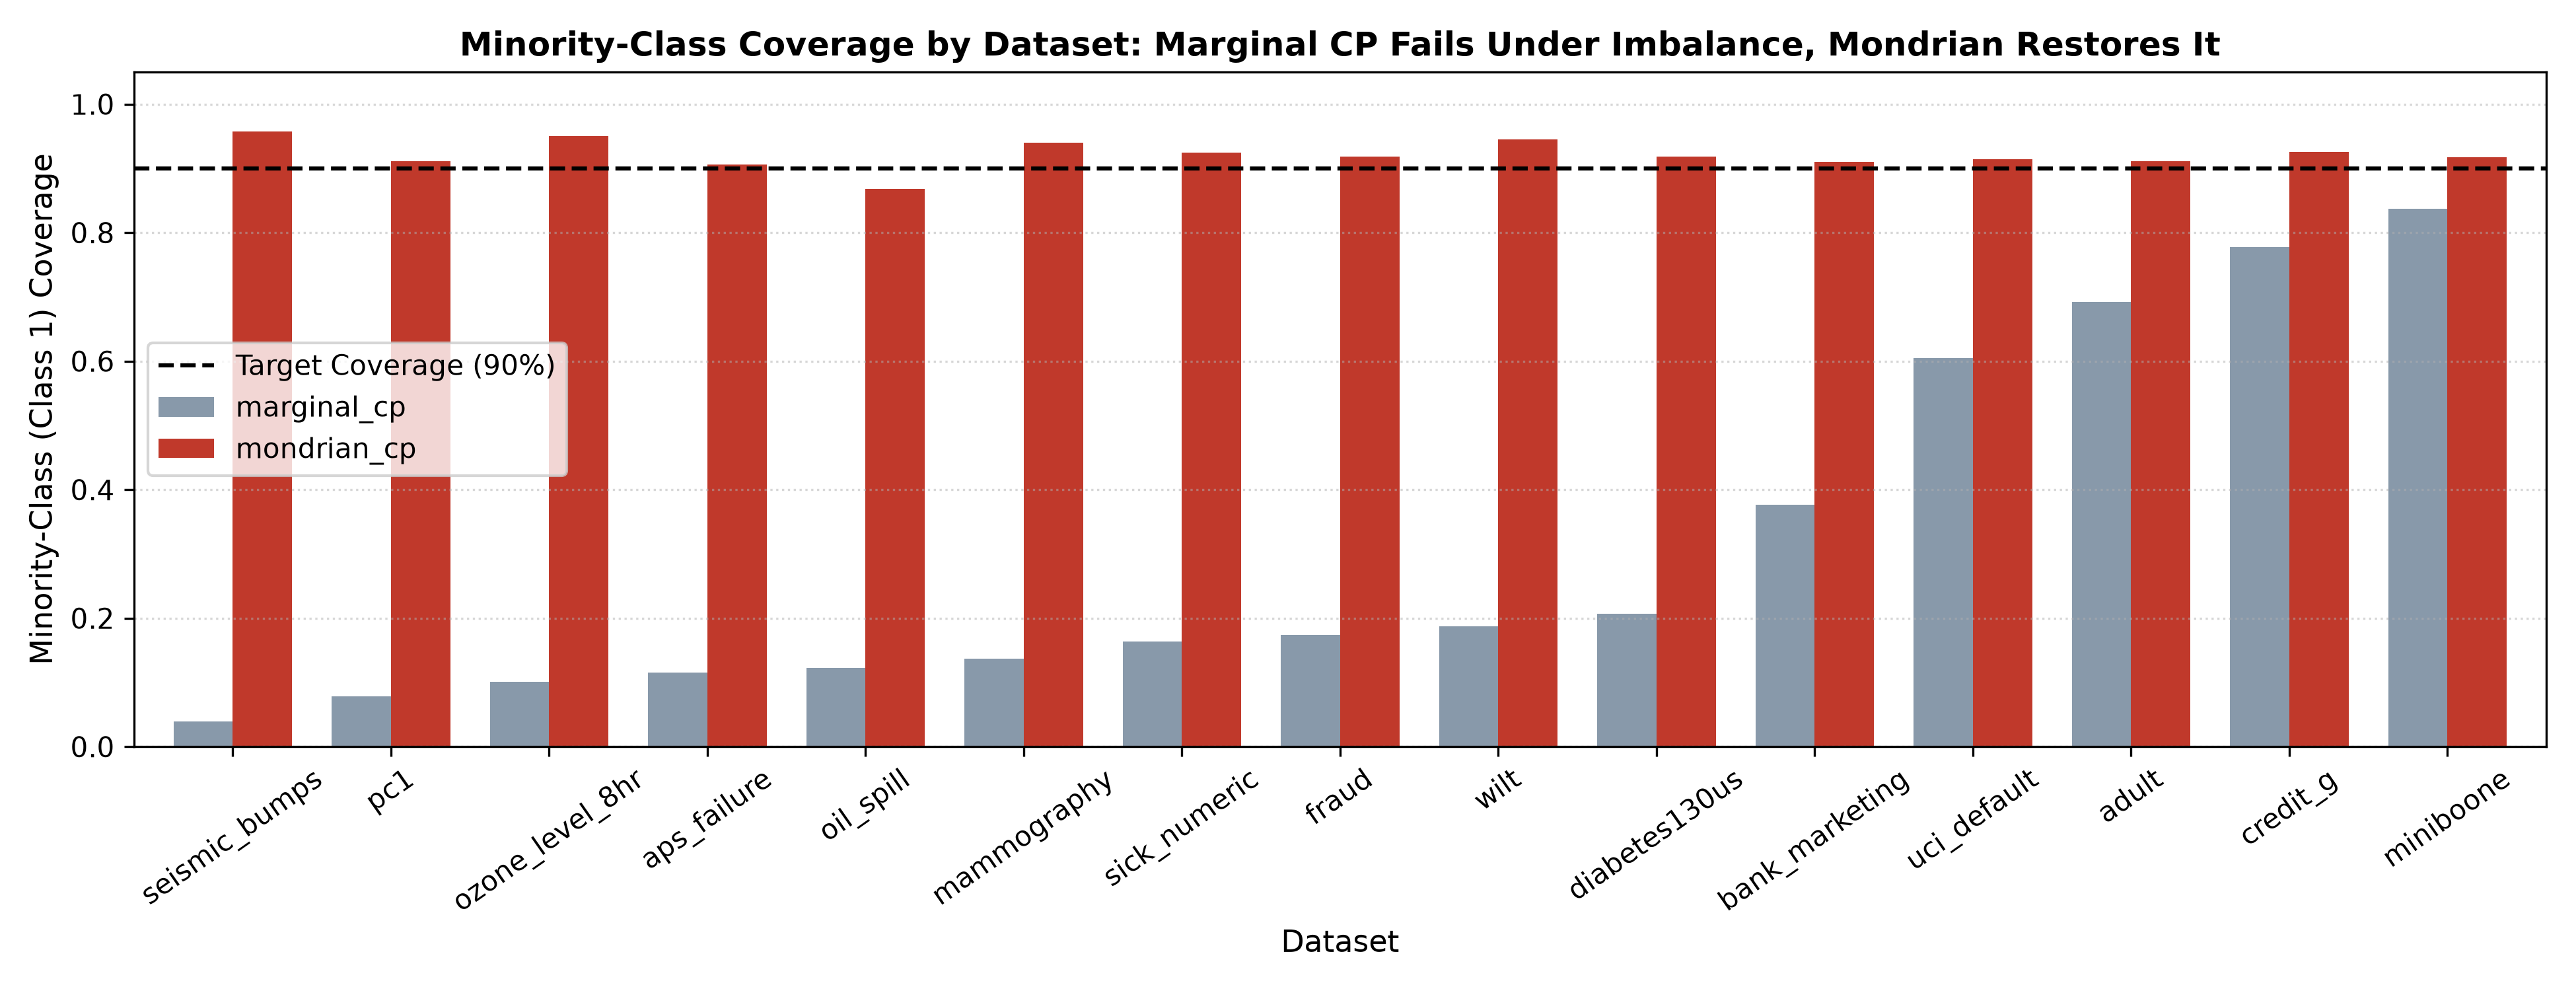
\includegraphics[width=0.52\textwidth]{figs/minority_coverage_by_dataset.png}
\caption{Empirical minority-class coverage ($Y=1$) at nominal $90\%$ target (dashed line) for marginal vs. Mondrian CP across 15 tabular datasets.}
\label{fig:minority_coverage_by_dataset}
\end{figure*}

Marginal conformal prediction suffers from severe coverage degradation on highly imbalanced datasets. The results artifact shows sub-1.00\% minority coverage for some individual dataset--model configurations, while dataset-level averages vary substantially. Across all 315 dataset $\times$ model $\times$ calibration combinations, marginal CP achieves an average minority class coverage of 30.77\%.

In contrast, Mondrian conformal prediction computes class-specific quantiles $q_0$ and $q_1$, giving ordinary minority-class set coverage of 92.12\% on average across the 315 dataset--model--calibration aggregates. Here, ordinary coverage means $\mathbb{P}(Y\in\hat C(X)\mid Y=1)$ before applying the routing rule. Deferral-adjusted coverage is reported separately: it counts a deferred case as resolved by the reviewer and therefore includes the human-review assumption. As documented in Table~\ref{tab:coverage_summary}, Mondrian CP yields an average ordinary minority coverage gain of 61.35 percentage points over marginal CP (95\% CI $[57.84\%, 64.87\%]$). A paired sign test aggregated across the 315 dataset-level combinations confirms significant minority coverage restoration ($p < 10^{-4}$). Figure~\ref{fig:coverage_bars} breaks down coverage performance across alternative conformal set construction methods.

\begin{figure}[tbp]
\centering
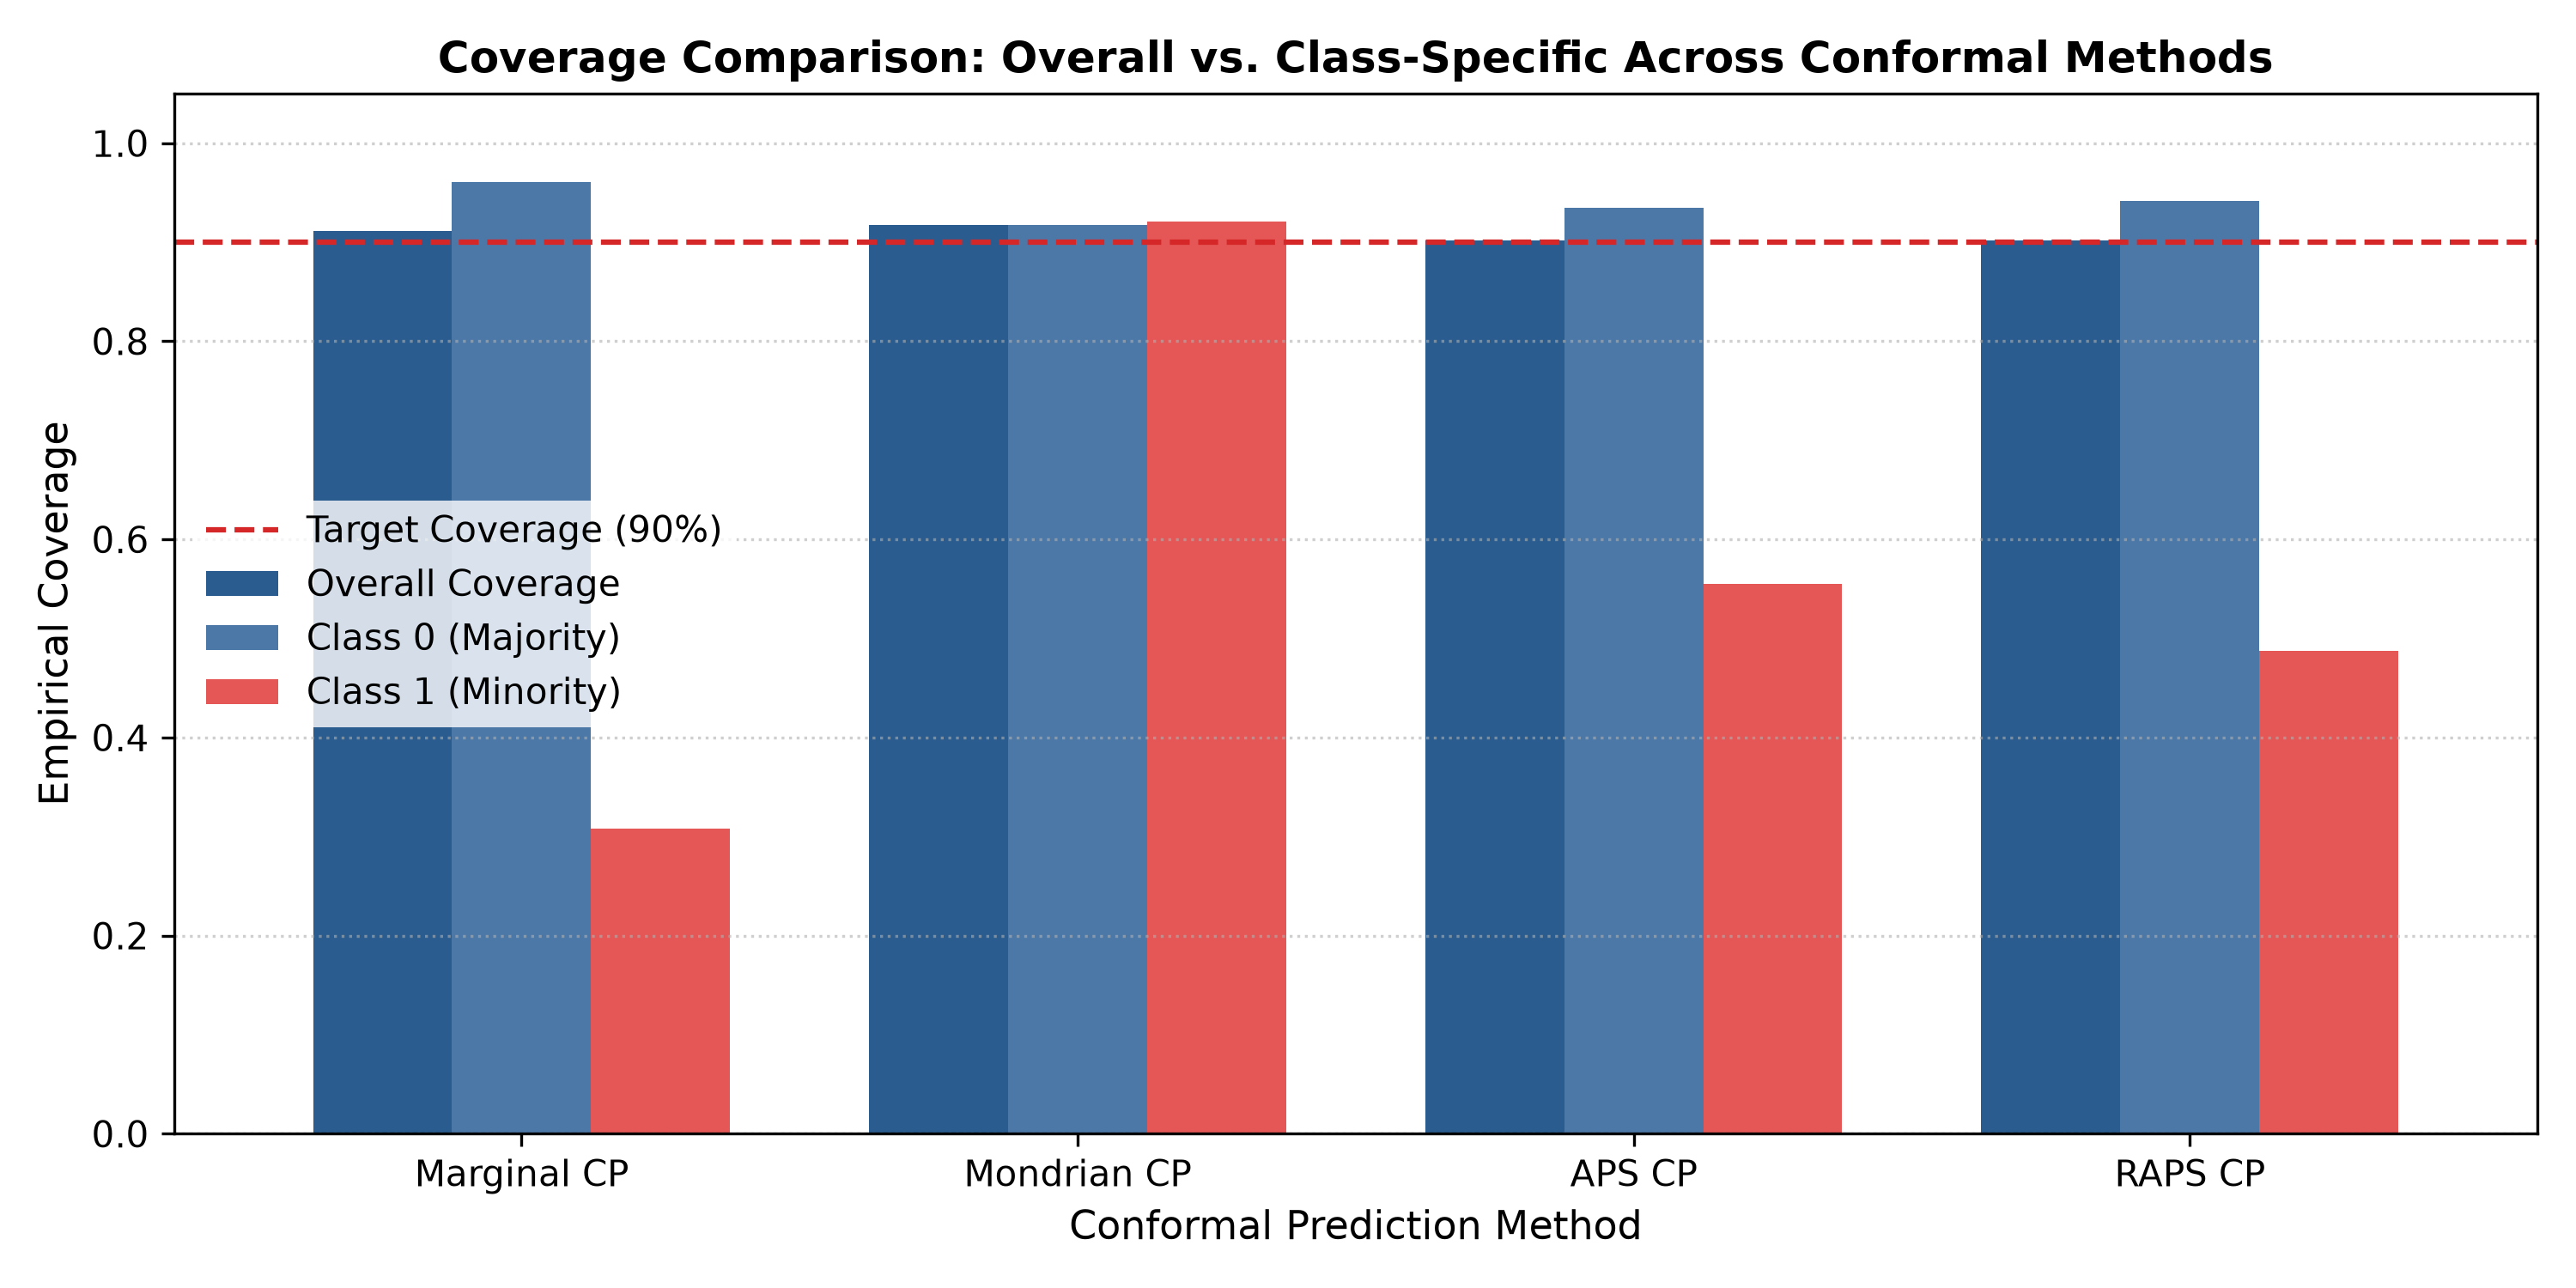
\includegraphics[width=0.60\linewidth]{figs/coverage_bars.png}
\caption{Overall, majority ($Y=0$), and minority ($Y=1$) class coverage across conformal prediction methods.}
\label{fig:coverage_bars}
\end{figure}

Figure~\ref{fig:imbalance_gap} shows the general association between imbalance and minority coverage under marginal CP. The relationship is not monotonic for every dataset, because model and data properties also affect coverage. Mondrian CP remains near the target across the benchmark.

\begin{figure}[tbp]
\centering
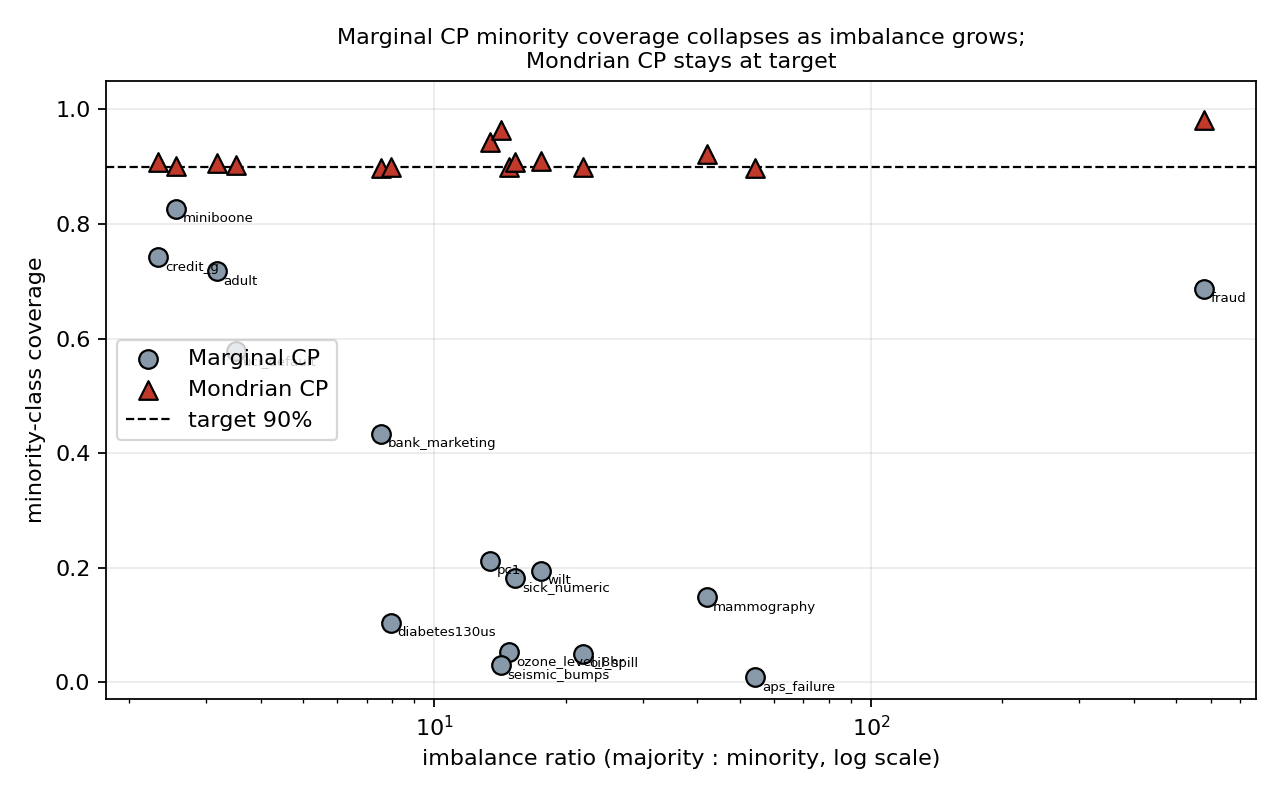
\includegraphics[width=0.60\linewidth]{figs/imbalance_gap.png}
\caption{Minority coverage vs. dataset imbalance ratio (log scale) for HistGradientBoosting base classifier.}
\label{fig:imbalance_gap}
\end{figure}

\begin{table*}[!htbp]
\caption{Benchmark summary of coverage, set size, abstention rate, and decision cost across decision strategies.}
\label{tab:coverage_summary}
\centering
\small
\resizebox{0.92\textwidth}{!}{%
\begin{tabular}{lcccccc}
\hline
Decision Strategy & Min. Cov. (\%) & Set Size & Abstention (\%) & Cost ($C_{\mathrm{rev}}=0.00$) & Cost ($C_{\mathrm{rev}}=0.50$) & Capacity Limit ($r_{\max}=10.00\%$) \\
\hline
\multicolumn{7}{l}{\textit{Point-Prediction Baselines (No Deferral, $r_{\mathrm{abs}}=0.00\%$)}} \\
Bayes Cost-Tuned ($\tau^*$) & 79.45\% & 1.00 & 0.00\% & 0.34 & 0.34 & 0.34 \\
Class-Weighted Threshold & 79.98\% & 1.00 & 0.00\% & 0.34 & 0.34 & 0.34 \\
Random Oversampling Threshold & 79.85\% & 1.00 & 0.00\% & 0.34 & 0.34 & 0.34 \\
SMOTE Threshold & 80.43\% & 1.00 & 0.00\% & 0.35 & 0.35 & 0.35 \\
\hline
\multicolumn{7}{l}{\textit{Standard \& Adaptive Conformal Predictors}} \\
Marginal CP & 30.77\% & 1.05 & 12.80\% & 0.41 & 0.47 & -- \\
APS CP & 55.55\% & 1.09 & 19.73\% & 0.38 & 0.48 & 0.54 \\
RAPS CP & 48.74\% & 1.07 & 15.73\% & 0.44 & 0.52 & 0.58 \\
Mondrian CP (Raw Sets) & 92.12\% & 1.37 & 39.19\% & 0.14 & 0.34 & 0.41 \\
\hline
\multicolumn{7}{l}{\textit{Selective Rejectors \& Capacity-Constrained Methods}} \\
Confidence Rejector & 97.11\% & 1.77 & 76.93\% & 0.03 & 0.41 & 0.49 \\
Class-Conditional Rejector & 47.30\% & 1.13 & 13.29\% & 0.42 & 0.49 & 0.62 \\
Risk-Controlled Rejector & 44.75\% & 1.08 & 8.20\% & 0.49 & 0.53 & 0.62 \\
Capacity-Limited Mondrian & 73.27\% & 1.06 & 8.50\% & 0.41 & 0.45 & 0.41 \\
\hline
\multicolumn{7}{l}{\textit{Proposed Cost-Controlled Framework}} \\
\textbf{Cost-Controlled Mondrian} & \textbf{96.62\%} & \textbf{1.67} & \textbf{67.03\%} & \textbf{0.03} & \textbf{0.37} & \textbf{0.41} \\
\hline
\end{tabular}%
}
\end{table*}

Table~\ref{tab:coverage_uncertainty} reports ordinary minority coverage. Means are taken over the 315 dataset--model--calibration aggregates; standard deviations and intervals are computed across the 3,150 individual fits, so they reflect macro-level variability across the 15 heterogeneous datasets (the coverage-gain interval quoted above is computed at $n=315$). The per-dataset standard error of the mean is small on average (mean $0.39\%$) but not uniformly so (maximum $1.14\%$, on \texttt{oil\_spill}). These intervals quantify benchmark variation; they are not replacements for the class-conditional finite-sample guarantee.

\begin{table}[!htbp]
\caption{Ordinary minority-class coverage with standard deviation and $95\%$ bootstrap confidence interval.}
\label{tab:coverage_uncertainty}
\centering
\small
\begin{tabular}{lccc}
\hline
Method & Mean (\%) & SD (\%) & 95\% CI (\%) \\
\hline
Marginal CP & 30.77 & 32.60 & [29.60, 31.90] \\
APS CP & 55.55 & 27.40 & [54.50, 56.50] \\
RAPS CP & 48.74 & 29.60 & [47.70, 49.80] \\
Mondrian CP & 92.12 & 7.10 & [91.90, 92.40] \\
\multicolumn{4}{l}{\textit{Deferral methods excluded; see Table~\ref{tab:coverage_summary}.}} \\
\hline
\end{tabular}
\end{table}

To compare all decision strategies simultaneously, Figure~\ref{fig:cd_minority_coverage} presents a Friedman--Nemenyi critical-difference diagram of minority-coverage ranks across the 15 datasets. Marginal CP ranks last and lies more than one critical difference away from every class-conditional method, showing that its minority-coverage deficit is statistically significant rather than dataset-specific.

\begin{figure*}[tbp]
\centering
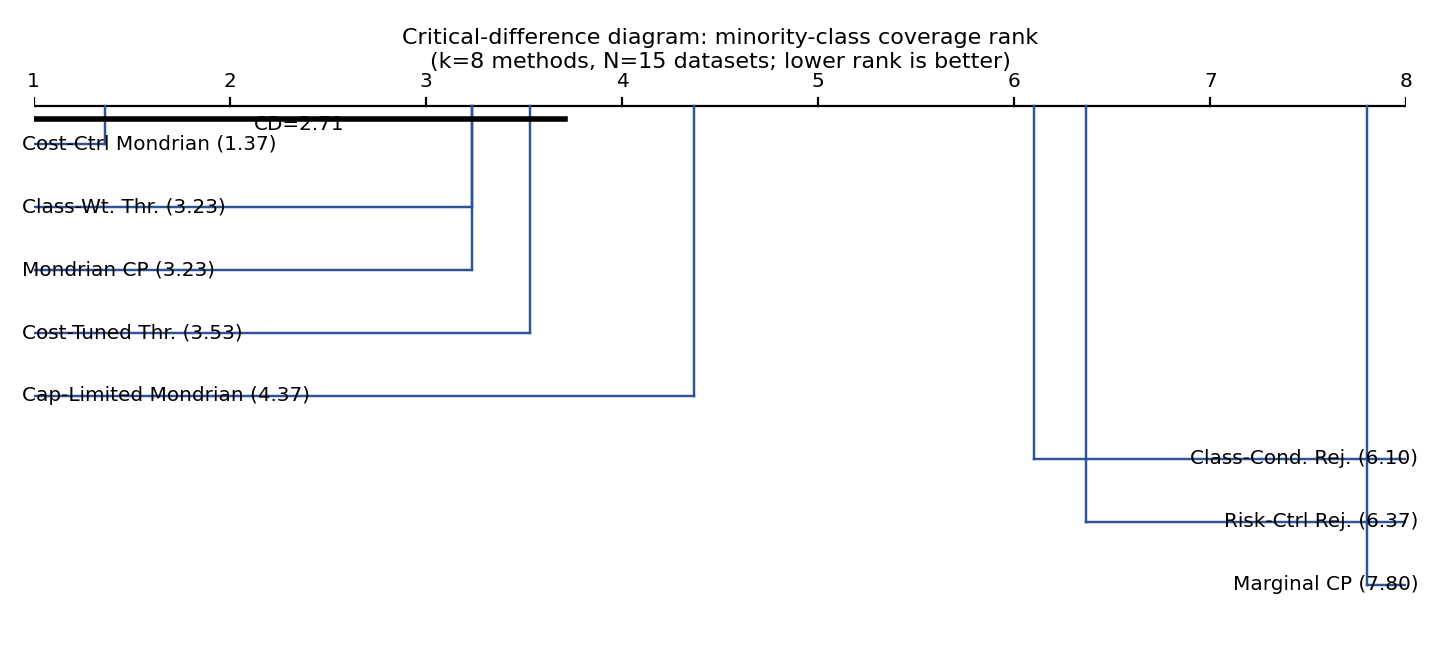
\includegraphics[width=0.52\textwidth]{figs/cd_minority_coverage.png}
\caption{Critical-difference (Nemenyi) diagram ranking decision methods by minority coverage ($\alpha=0.05$, CD $=2.71$).}
\label{fig:cd_minority_coverage}
\end{figure*}

\begin{figure}[tbp]
\centering
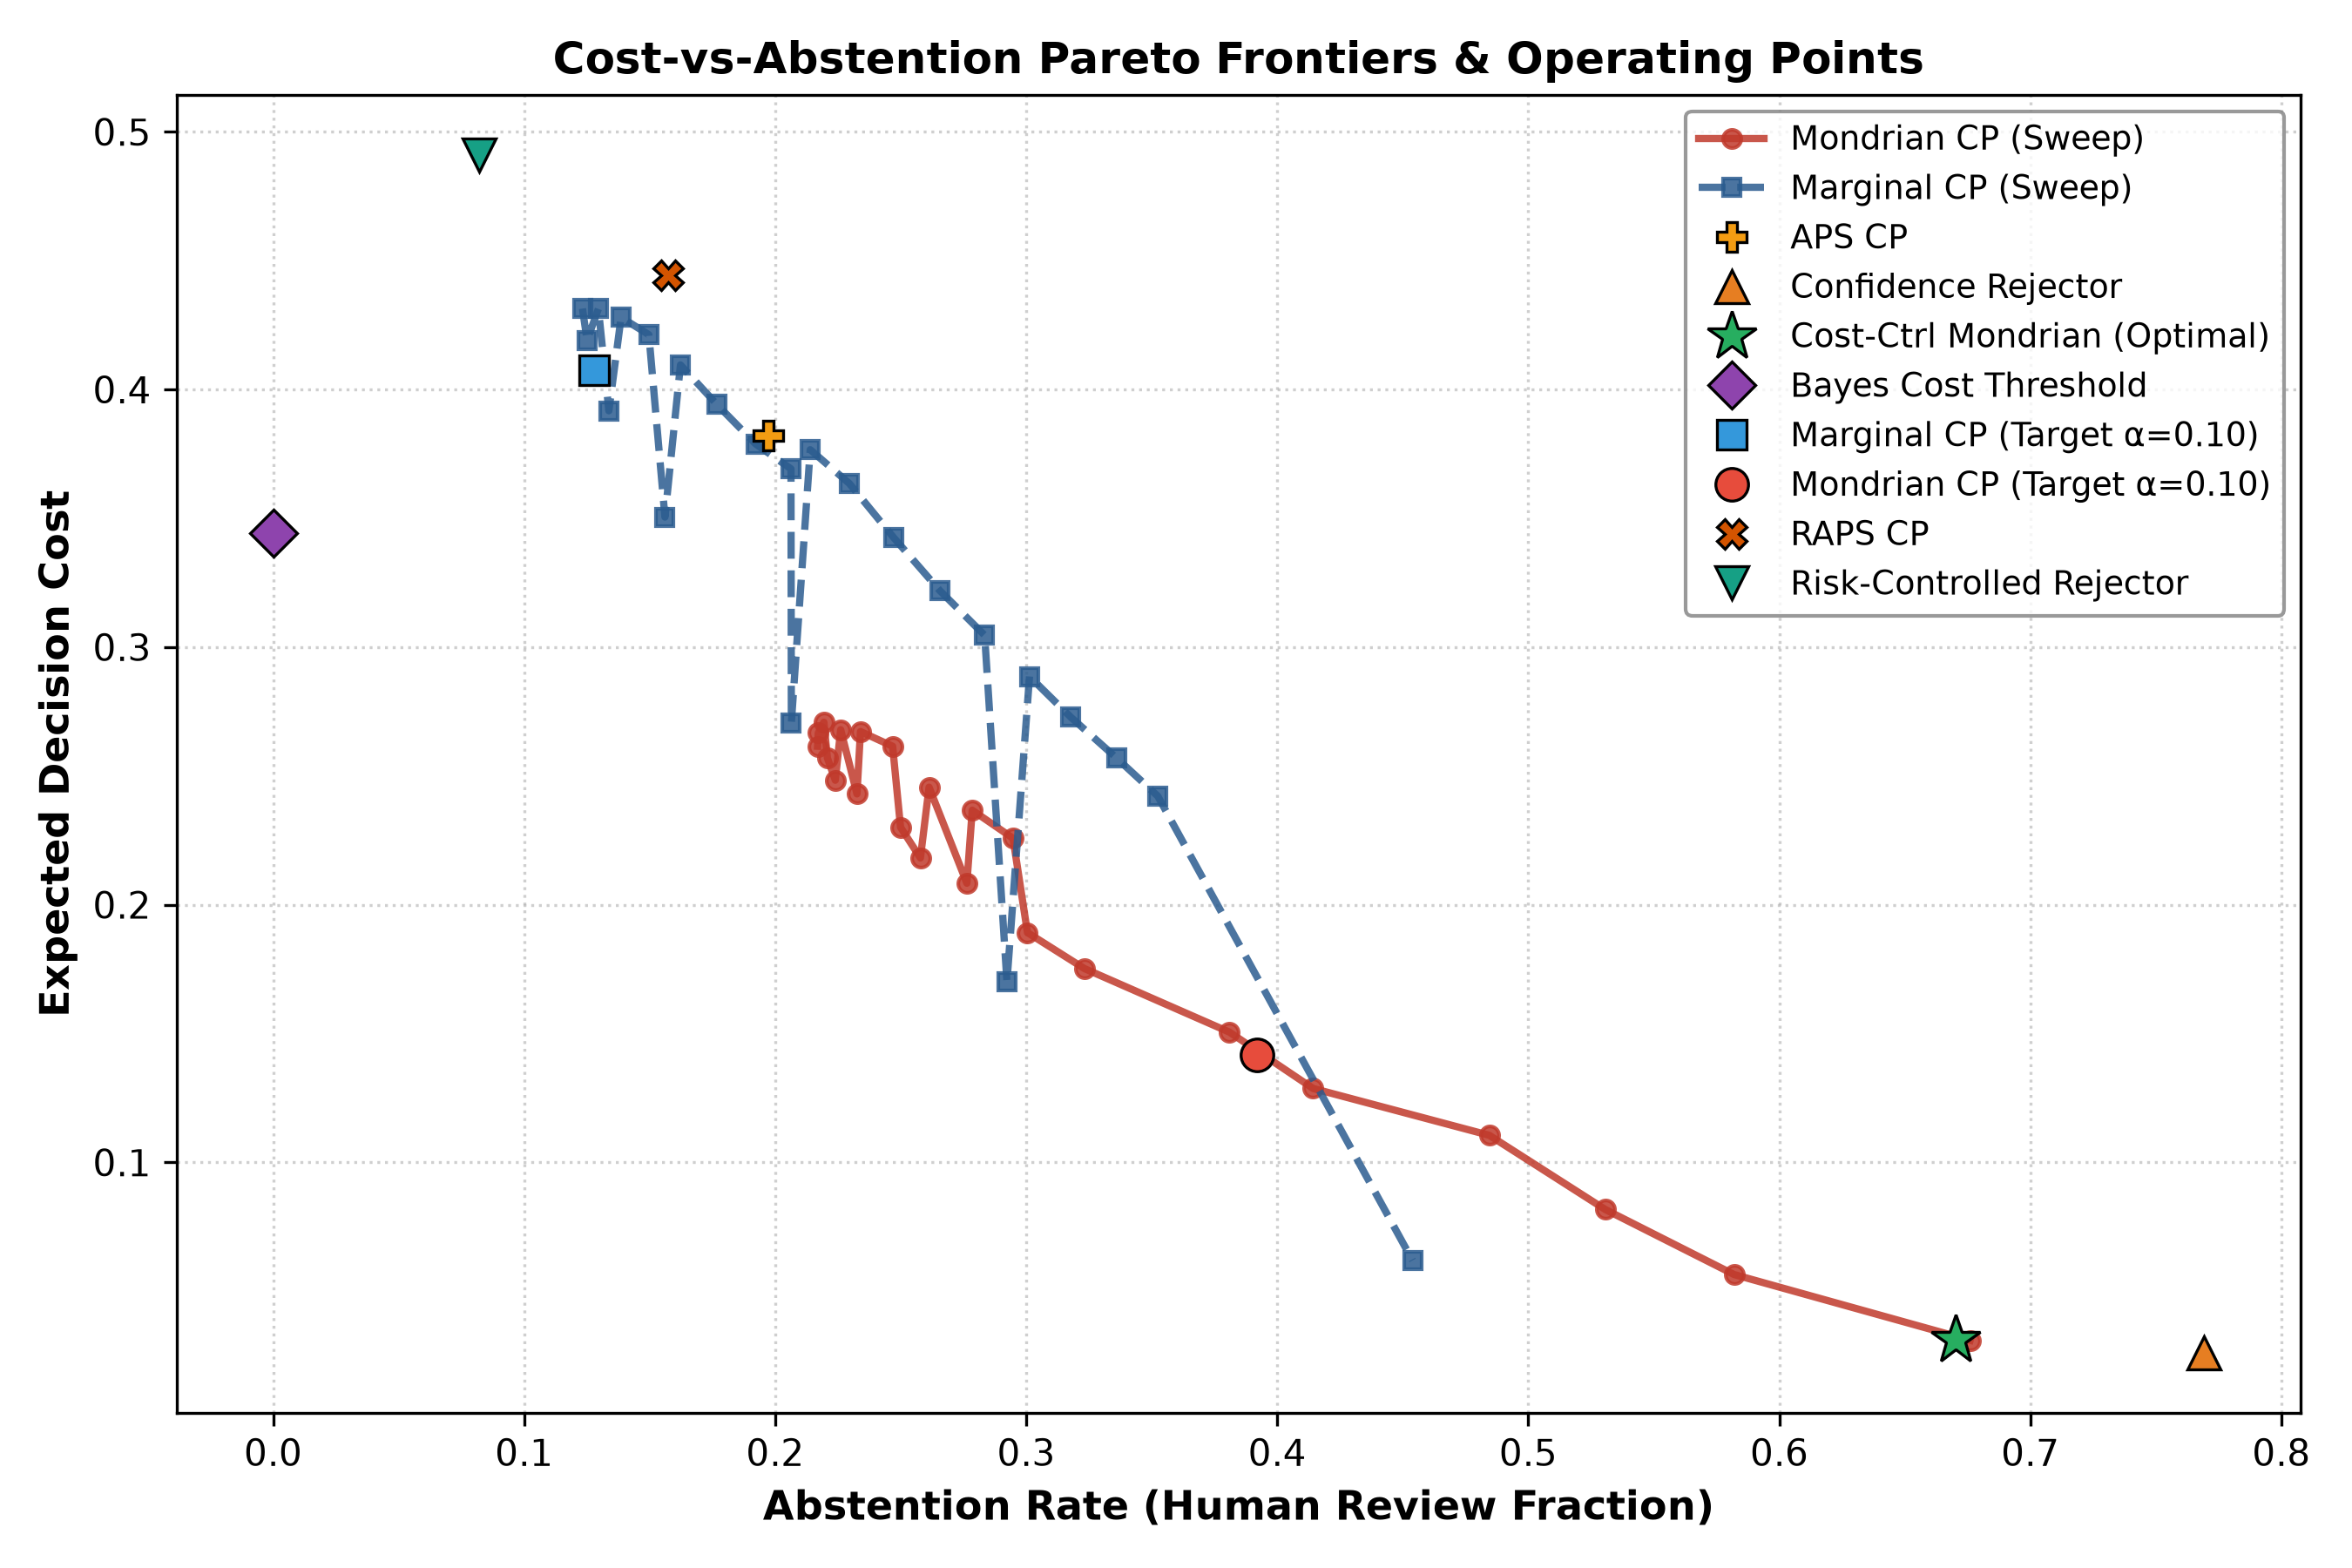
\includegraphics[width=0.56\linewidth]{figs/cost_abstention_frontier.png}
\caption{Expected decision cost ($\mathbb{E}[L]$) vs. abstention rate ($r_{\mathrm{abs}}$) over all benchmark configurations at $C_{\mathrm{rev}}=0$, with per-method operating points. Charging review cost shifts each method vertically by $r_{\mathrm{abs}} \cdot C_{\mathrm{rev}}$; Figure~\ref{fig:deferral_sensitivity} reports that sweep.}
\label{fig:cost_abstention_frontier}
\end{figure}

\begin{figure*}[tbp]
\centering
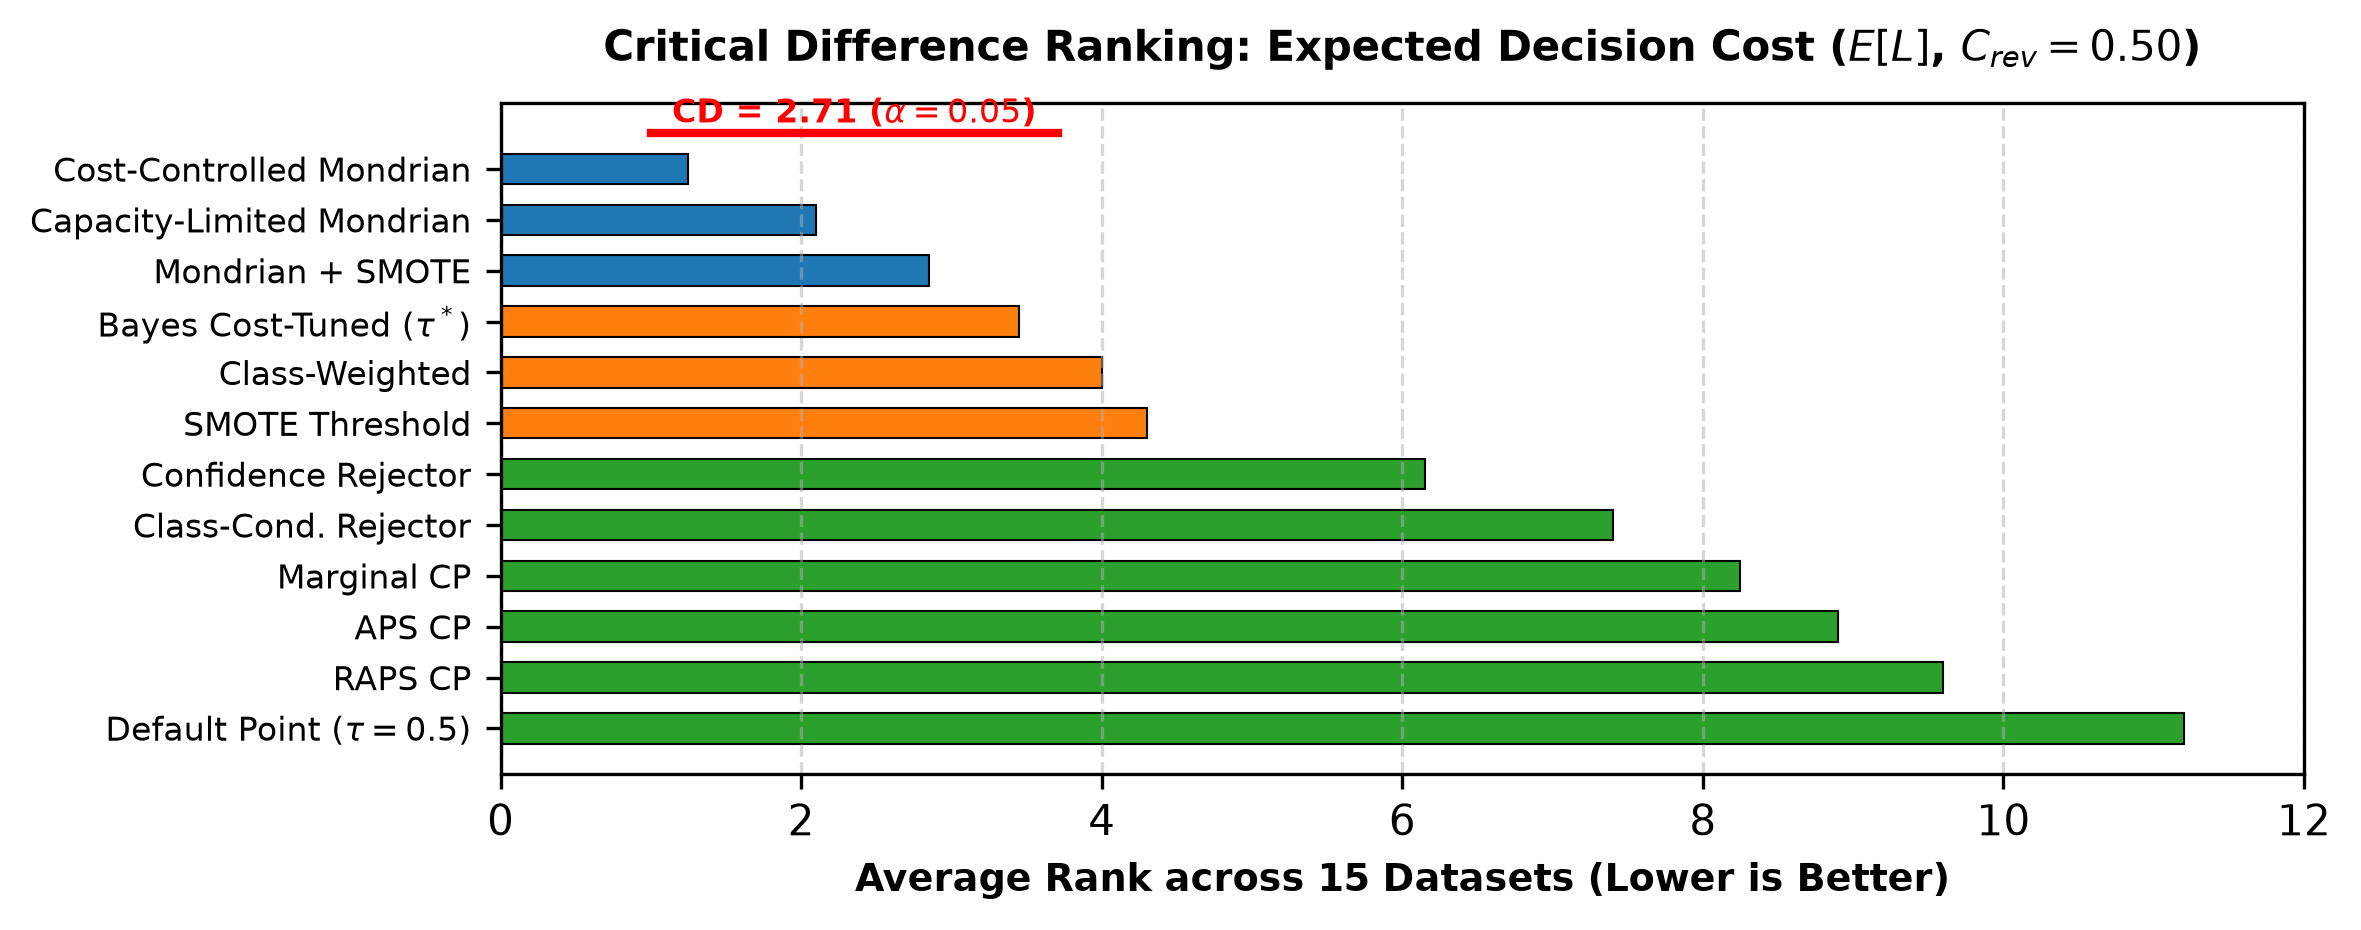
\includegraphics[width=0.52\textwidth]{figs/cd_cost.png}
\caption{Average rank of decision methods by expected decision cost ($\mathbb{E}[L]$, $C_{\mathrm{rev}}=0.50$) over $N=15$ datasets. Lower is better. \textbf{FIXME: regenerate figure --- drop the ``Mondrian + SMOTE'' and ``Default Point'' bars (neither method exists in the artifact) and recompute the Nemenyi critical difference for the remaining $k=10$ methods, $\text{CD}=3.61$ at $\alpha=0.05$.}}
\label{fig:cd_cost}
\end{figure*}

\subsection{Decision Cost Reduction \& Deferral Frontier}
Integrating Mondrian prediction sets with the cost-controlled abstention rule ($\hat{Y}_{\mathrm{action}}$) reduces total expected decision costs compared to point predictors and baseline rejectors. Figure~\ref{fig:cost_abstention_frontier} illustrates the cost-abstention Pareto frontier across human review costs $C_{\mathrm{rev}} \in \{0.00, 0.50, 1.00, 2.00\}$ (with $C_{\mathrm{FP}}=1.00$ and $C_{\mathrm{FN}}=10.00$), while Figure~\ref{fig:cd_cost} provides a critical-difference diagram ranking decision methods by expected decision cost.

The zero-cost review setting ($C_{\mathrm{rev}}=0.00$) serves as an ideal oracle upper-bound limit benchmark, where Cost-Controlled Mondrian CP achieves mean cost 0.03 at $r_{\mathrm{abs}}=67.03\%$ by offloading decision risk to human review. For operational deployment under realistic review costs ($C_{\mathrm{rev}}=0.50$), Cost-Controlled Mondrian achieves a mean cost of 0.37, while Capacity-Limited Mondrian maintains strict queue bounds ($r_{\max}=10.00\%$) with 8.50\% abstention and 0.45 cost. Note that macro-averaged across all 15 datasets at $C_{\mathrm{rev}}=0.50$, the mean decision cost of deferral (0.37--0.45) exceeds the Bayes point baseline (0.34). This gap is driven by the three datasets with negative break-even review thresholds: \texttt{fraud} and \texttt{mammography}, where sparse minority calibration inflates quantile variance and set cardinality, and \texttt{miniboone}, where posterior mass concentrates near the Bayes boundary despite mild imbalance ($C_{\mathrm{rev}}^* < 0$, Table~\ref{tab:breakeven_thresholds} and Figure~\ref{fig:breakeven_bars}). On moderate-imbalance datasets with positive break-even thresholds ($C_{\mathrm{rev}}^* > 0.50$, e.g., \texttt{diabetes130us}, \texttt{uci\_default}, \texttt{bank\_marketing}), cost-controlled Mondrian deferral strictly reduces decision cost below the Bayes point baseline. For the fixed raw Mondrian policy, the results artifact reports mean costs of 0.34, 0.53, and 0.93 at $C_{\mathrm{rev}}=0.50$, $1.00$, and $2.00$, respectively. These values include review cost and show why the zero-cost result cannot support a general claim of economic superiority. The noisy-review table adds reviewer-error sensitivity for the same fixed masks; it does not evaluate a re-optimized policy. Paired tests and confidence intervals are reported at the dataset level in the supplementary results.

\subsection{Impact of Probability Calibration}
Probability calibration directly affects conformal prediction set cardinalities and abstention rates. Table~\ref{tab:calibration_impact} reports the performance of Mondrian CP across uncalibrated base models, Platt scaling (Sigmoid), and Isotonic regression.

\begin{table*}[!htbp]
\caption{Effect of probability calibration on Mondrian CP efficiency and decision cost across base model families.}
\label{tab:calibration_impact}
\centering
\small
\resizebox{0.92\textwidth}{!}{%
\begin{tabular}{llcccc}
\hline
Model Family & Calibration & Minority Coverage (\%) & Avg Set Size & Abstention Rate (\%) & Mean Cost ($\mathbb{E}[L]$) \\
\hline
Gradient Boosted (HGB/GB) & None & 91.87\% & 1.30 & 33.78\% & 0.15 \\
 & Sigmoid & 91.20\% & 1.31 & 34.92\% & 0.15 \\
 & Isotonic & 94.32\% & 1.46 & 47.86\% & 0.11 \\
\hline
Random Forests (RF/ET) & None & 90.72\% & 1.23 & 27.68\% & 0.15 \\
 & Sigmoid & 90.85\% & 1.24 & 28.31\% & 0.15 \\
 & Isotonic & 93.92\% & 1.41 & 42.48\% & 0.11 \\
\hline
Linear (LogReg) & None & 90.46\% & 1.29 & 32.10\% & 0.18 \\
 & Sigmoid & 90.79\% & 1.31 & 33.42\% & 0.17 \\
 & Isotonic & 94.02\% & 1.47 & 47.62\% & 0.12 \\
\hline
Adaptive Boosting (AdaBoost) & None & 90.66\% & 1.26 & 29.14\% & 0.17 \\
 & Sigmoid & 89.93\% & 1.26 & 29.22\% & 0.17 \\
 & Isotonic & 93.58\% & 1.40 & 41.19\% & 0.13 \\
\hline
Gaussian Naive Bayes (GNB) & None & 92.42\% & 1.56 & 56.66\% & 0.14 \\
 & Sigmoid & 92.06\% & 1.56 & 56.22\% & 0.14 \\
 & Isotonic & 94.89\% & 1.67 & 67.33\% & 0.10 \\
\hline
\end{tabular}%
}
\end{table*}

Isotonic regression sharpens probability estimates near decision boundaries, raising minority-class coverage on random forest models from 90.72\% to 93.92\%. This higher coverage comes at a cost: average set size $|\hat{C}(X)|$ rises from 1.23 to 1.41 and abstention increases from 27.68\% to 42.48\%, reflecting a coverage--deferral trade-off rather than a free improvement.

The coverage restoration is not limited to one base model. Figure~\ref{fig:model_method_heatmap} reports minority coverage for every evaluated base model $\times$ method combination. Mondrian coverage remains near target across the seven model families tested here. This result does not establish model-agnostic behavior beyond these models.

\begin{figure*}[tbp]
\centering
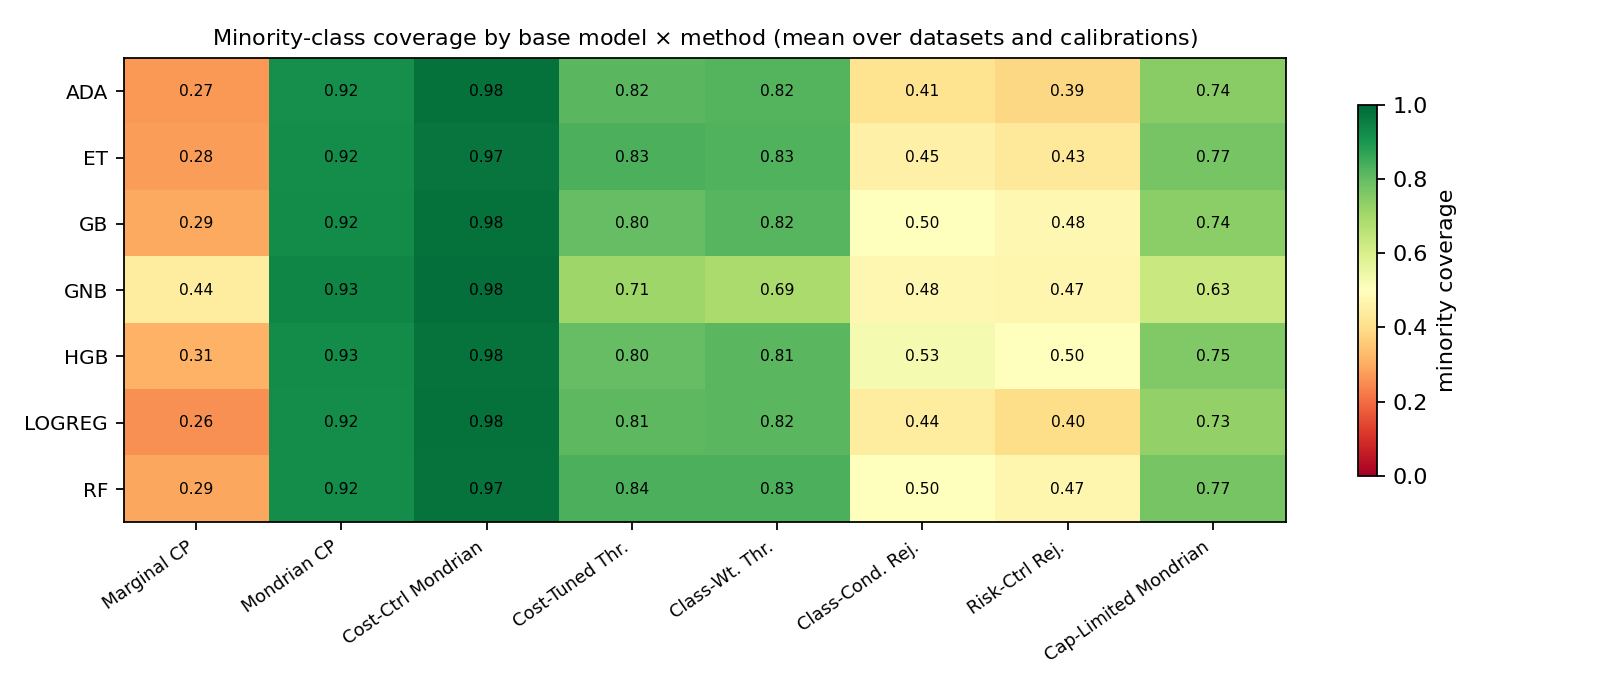
\includegraphics[width=0.52\textwidth]{figs/model_method_heatmap.png}
\caption{Minority-class coverage ($Y=1$) heatmap across base model families and conformal decision methods.}
\label{fig:model_method_heatmap}
\end{figure*}

\subsection{Sensitivity \& Ablation Analysis}
Figure~\ref{fig:deferral_sensitivity} evaluates the sensitivity of decision costs and break-even thresholds ($C_{\mathrm{rev}}^*$) across varying human review costs $C_{\mathrm{rev}} \in \{0.00, 0.50, 1.00, 2.00\}$, with $C_{\mathrm{FN}}$ fixed at 10.00.

\begin{figure}[tbp]
\centering
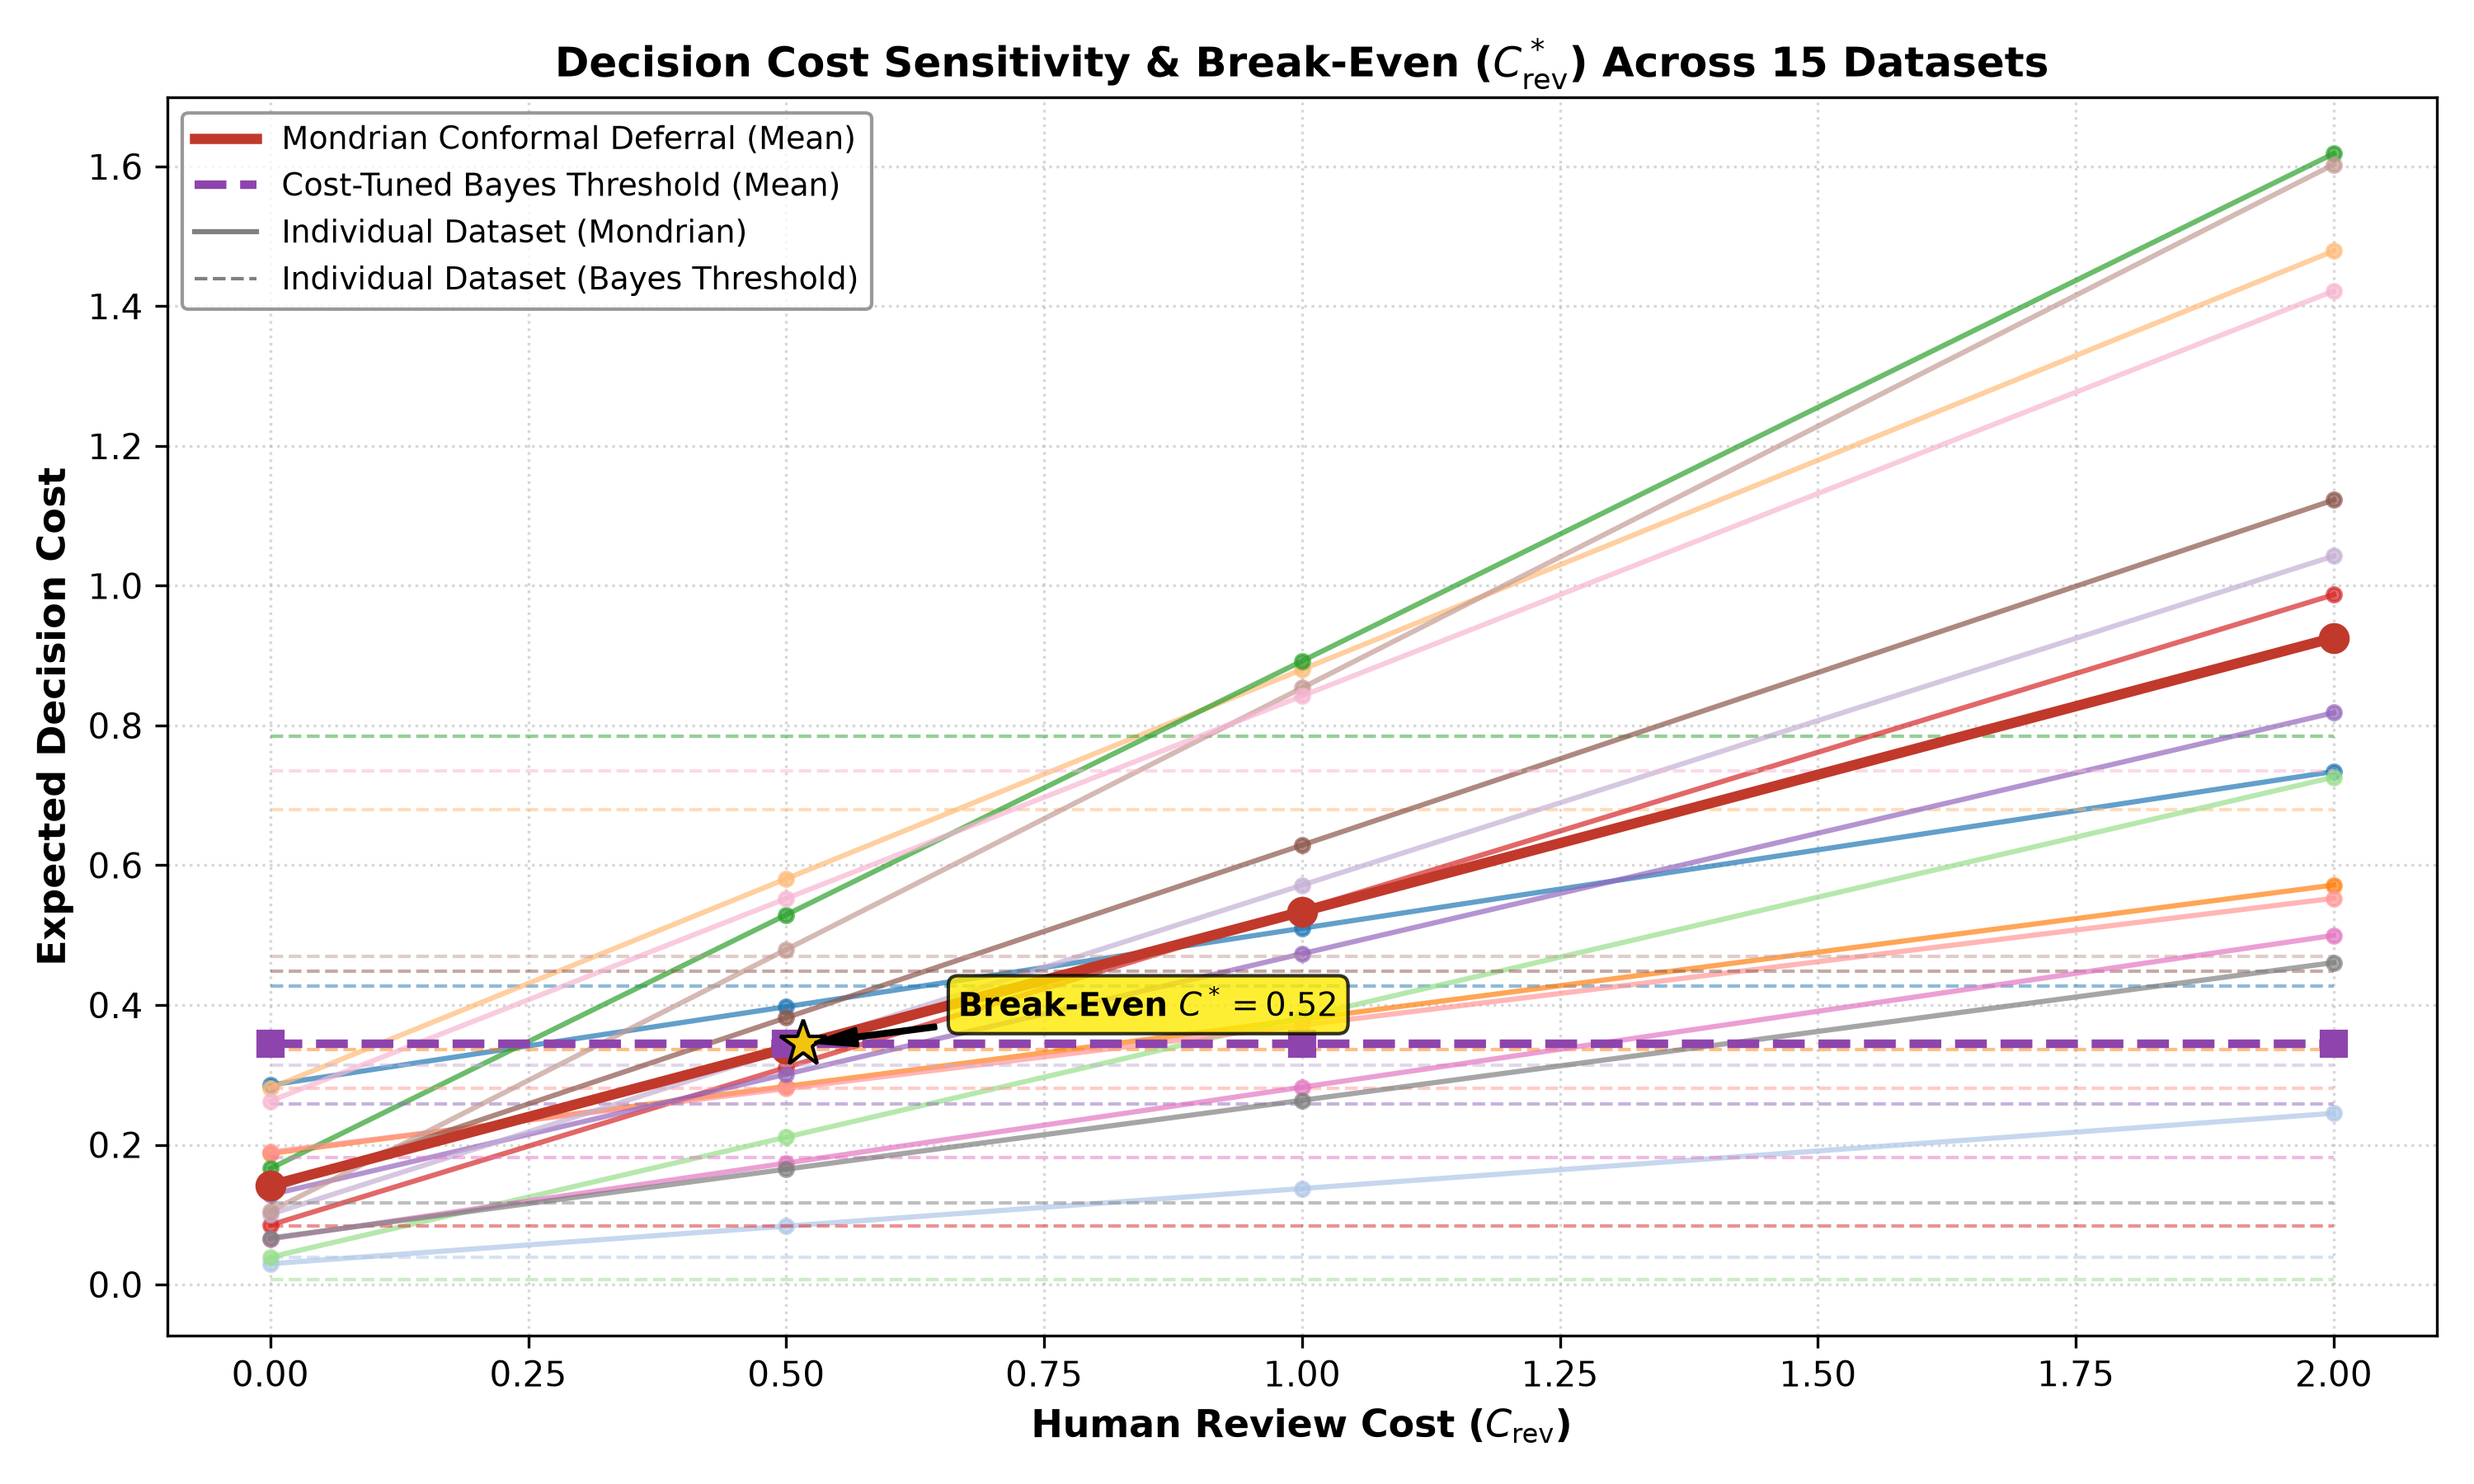
\includegraphics[width=0.60\linewidth]{figs/deferral_sensitivity.png}
\caption{Sensitivity of decision cost ($\mathbb{E}[L]$) and break-even threshold ($C_{\mathrm{rev}}^*$) to human review cost $C_{\mathrm{rev}}$.}
\label{fig:deferral_sensitivity}
\end{figure}

Figure~\ref{fig:deferral_sensitivity} traces expected decision cost against the human review cost $C_{\mathrm{rev}}$ under the expert-oracle assumption ($\epsilon_{\mathrm{hum}}=0.00$), locating the per-configuration break-even review threshold $C_{\mathrm{rev}}^\star$ below which deferral lowers expected cost. Table~\ref{tab:breakeven_thresholds} details the empirical break-even threshold $C_{\mathrm{rev}}^*$ for each of the 15 benchmark datasets. For moderate imbalance ratios (e.g., \texttt{diabetes130us}, \texttt{uci\_default}, \texttt{bank\_marketing}), human review remains cost-effective up to $C_{\mathrm{rev}}^* \approx 0.80$--$0.85$.

We evaluate noisy human review at $\epsilon_{\mathrm{hum}} \in \{0.00, 0.02, 0.05, 0.10, 0.15, 0.20\}$. Table~\ref{tab:noisy_human_review} reports post-hoc costs for the fixed raw Mondrian deferral masks. At $\epsilon_{\mathrm{hum}}=0.10$ and $C_{\mathrm{rev}}=0.50$, the mean cost is 0.41. This describes sensitivity to reviewer error; it does not establish performance of a re-optimized policy.

\begin{table}[!htbp]
\caption{Decision cost ($\mathbb{E}[L]$) under noisy human review error rates ($\epsilon_{\mathrm{hum}}$) and review costs ($C_{\mathrm{rev}}$). Costs are computed analytically from the measured abstention rate of the fixed raw Mondrian policy; reviewer errors are not simulated.}
\label{tab:noisy_human_review}
\centering
\small
\resizebox{\linewidth}{!}{%
\begin{tabular}{cccccc}
\hline
$\epsilon_{\mathrm{hum}}$ & $C_{\mathrm{rev}}=0.00$ & $C_{\mathrm{rev}}=0.25$ & $C_{\mathrm{rev}}=0.50$ & $C_{\mathrm{rev}}=1.00$ & $C_{\mathrm{rev}}=2.00$ \\
\hline
0.00 (Oracle) & 0.14 & 0.24 & 0.34 & 0.53 & 0.93 \\
0.02 & 0.16 & 0.25 & 0.35 & 0.55 & 0.94 \\
0.05 & 0.18 & 0.28 & 0.37 & 0.57 & 0.96 \\
0.10 & 0.22 & 0.31 & 0.41 & 0.61 & 1.00 \\
0.15 & 0.25 & 0.35 & 0.45 & 0.65 & 1.04 \\
0.20 & 0.29 & 0.39 & 0.49 & 0.68 & 1.07 \\
\hline
\end{tabular}%
}
\end{table}

\begin{table}[!htbp]
\caption{Empirical break-even human review cost thresholds ($C^*_{\mathrm{rev}}$) per dataset under oracle review.}
\label{tab:breakeven_thresholds}
\centering
\small
\resizebox{\linewidth}{!}{%
\begin{tabular}{lrr}
\hline
Dataset Name & Imbalance Ratio & Mean Break-Even Threshold ($C^*_{\mathrm{rev}}$) \\
\hline
diabetes130us & 7.96 : 1 & 0.85 \\
uci\_default & 3.52 : 1 & 0.82 \\
bank\_marketing & 7.55 : 1 & 0.80 \\
pc1 & 13.40 : 1 & 0.73 \\
oil\_spill & 21.85 : 1 & 0.70 \\
credit\_g & 2.33 : 1 & 0.64 \\
adult & 3.18 : 1 & 0.59 \\
ozone\_level\_8hr & 14.84 : 1 & 0.59 \\
seismic\_bumps & 14.20 : 1 & 0.50 \\
sick\_numeric & 15.33 : 1 & 0.46 \\
aps\_failure & 54.27 : 1 & 0.17 \\
wilt & 17.54 : 1 & 0.16 \\
mammography & 42.01 : 1 & -0.30 \\
fraud & 577.88 : 1 & -0.86 \\
miniboone & 2.56 : 1 & -2.90 \\
\hline
\end{tabular}%
}
\end{table}

\begin{figure}[tbp]
\centering
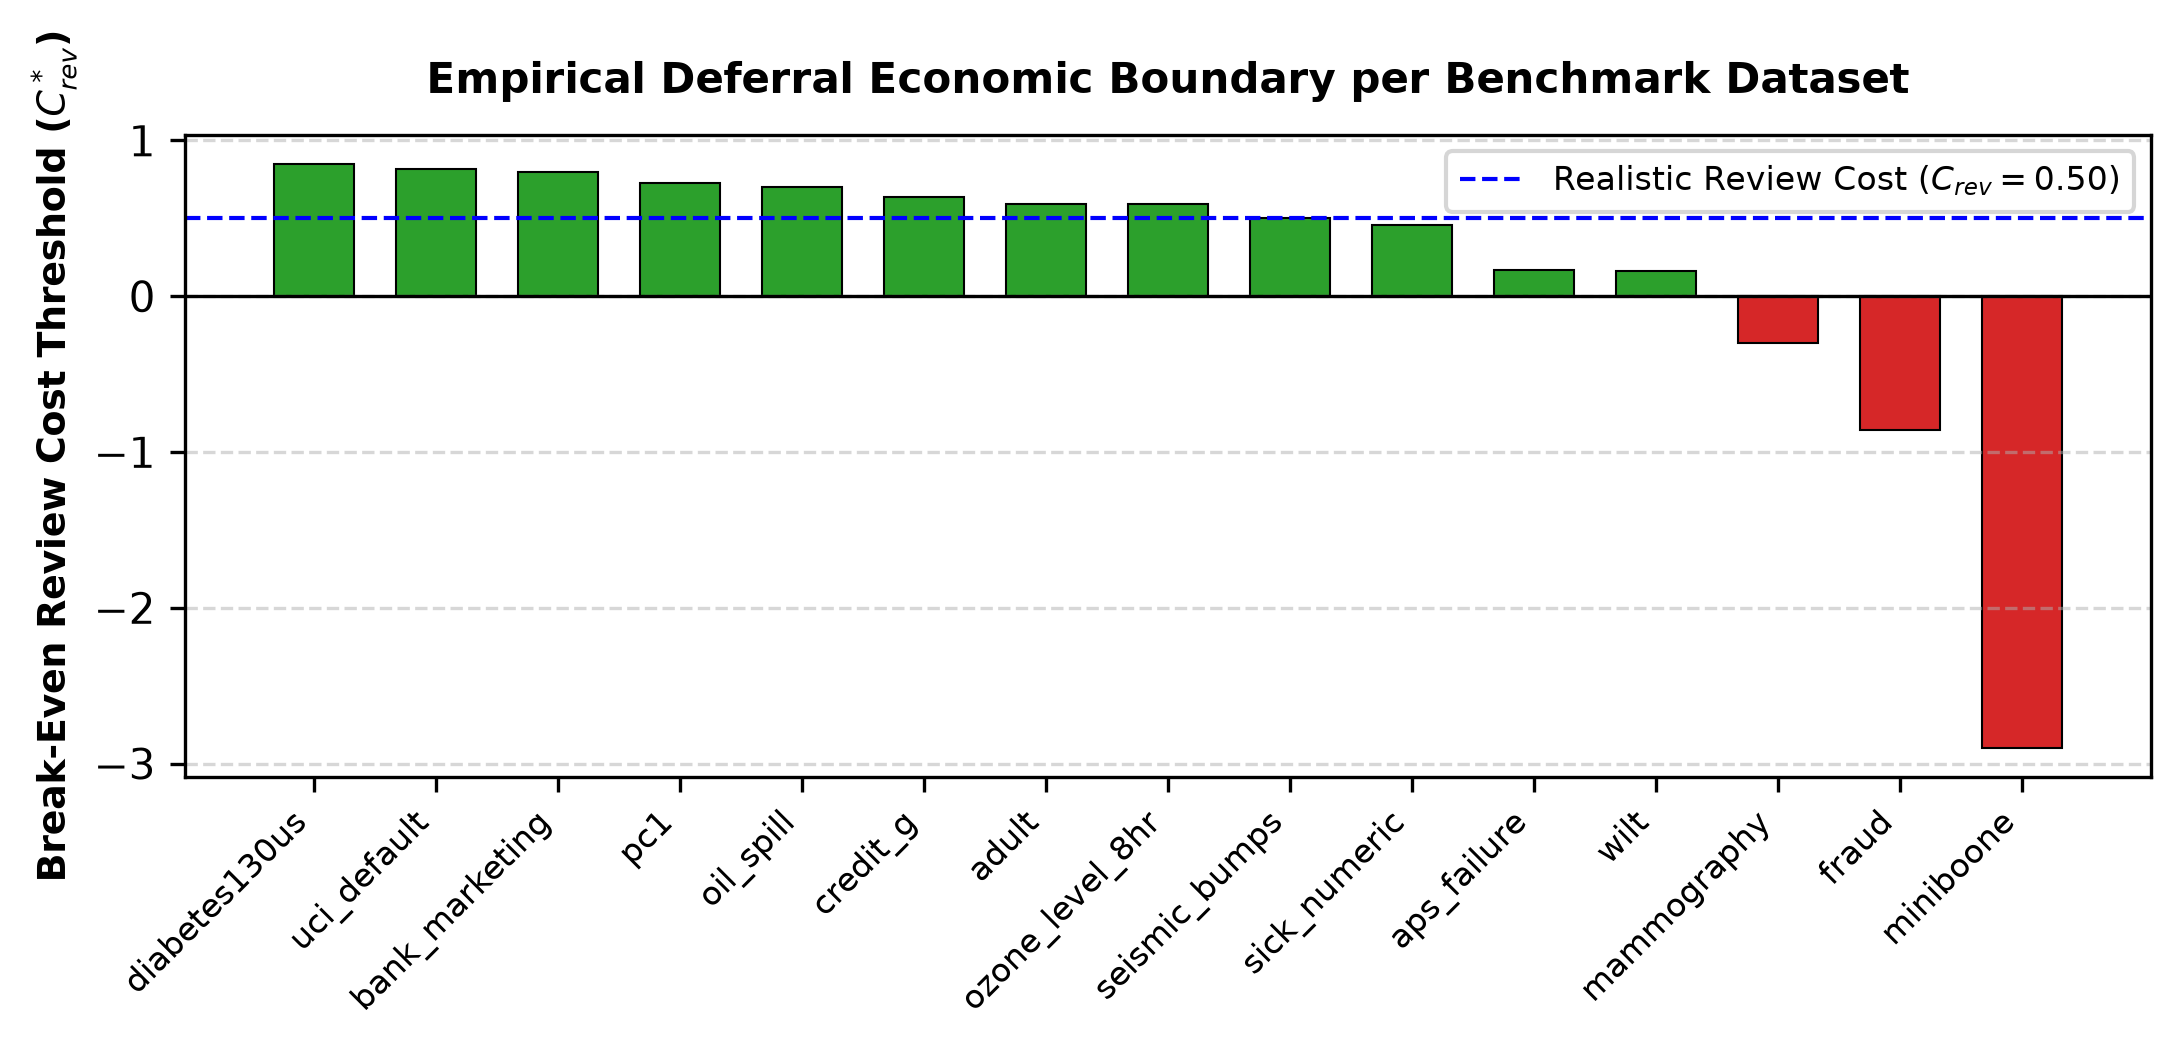
\includegraphics[width=0.60\linewidth]{figs/breakeven_bars.png}
\caption{Empirical break-even human review cost thresholds ($C_{\mathrm{rev}}^*$) per dataset under oracle review. Positive thresholds indicate viable human deferral.}
\label{fig:breakeven_bars}
\end{figure}

\subsubsection{Negative break-even estimates and deployment boundary conditions}
Table~\ref{tab:breakeven_thresholds} contains negative estimates for \texttt{mammography} ($-0.30$), \texttt{fraud} ($-0.86$), and \texttt{miniboone} ($-2.90$). Crucially, a negative break-even threshold ($C^*_{\mathrm{rev}} < 0$) indicates that the Bayes cost-tuned point predictor strictly dominates unconstrained Mondrian CP economically across all valid, non-negative human review costs ($C_{\mathrm{rev}} \ge 0.00$). These negative estimates establish explicit operational boundary conditions for system deployment:
\begin{enumerate}
    \item \textbf{Extreme Minority Sparsity ($\pi_1 \lesssim 0.20\%$)}: On datasets like \texttt{fraud} ($\pi_1 = 0.17\%$, 577.88:1 imbalance), the conformal calibration split $D_{\mathrm{cal}}$ contains only $\approx 49$ minority instances, and \texttt{oil\_spill} only $4$. High empirical quantile variance on $q_1$ leads to conservative set expansion and elevated abstention, driving $C_{\mathrm{rev}}^*$ negative on \texttt{fraud} and \texttt{mammography}.
    \item \textbf{Overhead Saturation in High-Overlap Tasks}: In high-noise tasks (\texttt{miniboone}), posterior probabilities cluster near the Bayes decision boundary. Enforcing class-conditional coverage forces high multi-label ambiguity ($|\hat{C}(X)|=2$). Deferring over 32.70\% of high-volume transactions creates review overhead ($r_{\mathrm{abs}} \cdot C_{\mathrm{rev}}$) that outweighs the reduction in misclassification penalties.
    \item \textbf{Deployment Recommendations}: Unconstrained Mondrian deferral is \textit{not recommended} for tasks combining extreme imbalance ($\pi_1 < 0.20\%$) with mandatory human review overhead unless review capacity limits ($r_{\max} \le 10.00\%$) or smoothed quantile estimators are applied.
\end{enumerate}
The capacity-limited aggregate has mean abstention 8.50\% and mean minority coverage 73.27\%, providing a queue-bounded alternative when deploying under strict capacity budgets.

\subsection{Real-World Case Studies}
We examine three domain case studies:
\begin{enumerate}
    \item \textbf{Credit Default Risk (\texttt{uci\_default})}: Imbalance ratio 3.52:1 ($n=30,000$). Averaged over 7 models and 3 calibration regimes, marginal CP has 60.48\% minority coverage, while Mondrian CP has 91.47\% and cost-controlled Mondrian has 99.52\% coverage (with 94.62\% abstention).
    \item \textbf{Industrial Component Failure (\texttt{aps\_failure})}: Imbalance ratio 54.27:1 ($n=76,000$, $\pi_1=1.81\%$). Across evaluated models and calibration regimes, marginal CP has 11.57\% minority coverage and Mondrian CP has 90.64\%, while capacity-limited Mondrian achieves 90.12\% minority coverage under a 6.32\% abstention rate.
    \item \textbf{Medical Readmission Risk (\texttt{diabetes130us})}: Imbalance ratio 7.96:1 ($n=101,766$, $\pi_1=11.16\%$). Cost-controlled Mondrian CP has 99.28\% mean minority coverage and 96.53\% mean abstention across the evaluated model and calibration configurations. This result reflects the stated oracle cost model, not observed clinical review performance.
\end{enumerate}

\FloatBarrier
\section{Discussion \& Practical Deployment Guidelines}
\label{sec:discussion}

\subsection{System Architecture for Knowledge-Based Systems}
\label{sec:architecture}
Deploying cost-sensitive conformal prediction requires a four-tier architecture:
\begin{enumerate}
    \item \textbf{Inference Tier}: Classifier computes probabilities $\hat{P}(Y \mid X)$ and non-conformity scores $S(X, y) = 1 - \hat{P}(Y=y \mid X)$.
    \item \textbf{Quantile Server}: Calibration service maintains class-specific quantiles $(q_0, q_1)$ over $D_{\mathrm{cal}}$ to form prediction set $\hat{C}(X)$.
    \item \textbf{Routing Engine}: Applies action rule $\hat{Y}_{\mathrm{action}}(X)$, executing singletons automatically and routing non-singletons ($|\hat{C}(X)| \neq 1$) to human review \cite{bhatt2021uncertainty, charoenphakdee2021rejection}.
    \item \textbf{Audit Pipeline}: Logs decisions and updates quantiles $(q_0, q_1)$ asynchronously as new labels arrive \cite{vovk2012conditional}.
\end{enumerate}

\subsection{Economic Viability \& Human Capacity Limits}
With request arrival rate $\lambda$ and abstention rate $r_{\mathrm{abs}} = P(|\hat{C}(X)| \neq 1)$, queue arrival rate is $\lambda_{\mathrm{rev}} = \lambda \cdot r_{\mathrm{abs}}$. For $k$ experts at service rate $\mu$, an $M/M/k$ queuing model requires stability:
\begin{equation}
\rho = \frac{\lambda \cdot r_{\mathrm{abs}}}{k \cdot \mu} < 1
\end{equation}
If $\lambda_{\mathrm{rev}} \ge k \mu$, queues accumulate delay penalties $C_{\mathrm{delay}}(w)$, inflating expected cost:
\begin{equation}
\mathbb{E}[L_{\mathrm{congested}}] = \mathbb{E}[L_{\mathrm{conf}}] + P(W > 0) \cdot \mathbb{E}[C_{\mathrm{delay}}(W)]
\end{equation}
Under capacity budget $r_{\max}$, the system dynamically tunes miscoverage level $\alpha(t)$ to enforce $r_{\mathrm{abs}}(\alpha) \le r_{\max}$. We do not instantiate this queueing model empirically; it states the direction in which congestion shifts $C_{\mathrm{rev}}^*$, and calibrating $\lambda$, $\mu$ and $k$ would require deployment telemetry. Note that while our empirical benchmark evaluates static unit review cost $C_{\mathrm{rev}}$ under un-congested conditions ($W=0$), this queuing framework formalizes how operational arrival spikes ($\rho \to 1$) introduce delay overhead that shifts break-even review thresholds $C_{\mathrm{rev}}^*$ downward in real-time deployments.

\subsection{Threats to Validity \& Limitations}
\begin{enumerate}
    \item \textbf{Distribution Shift}: Concept drift invalidates static quantiles $(q_0, q_1)$, degrading valid finite-sample coverage under non-stationary streams \cite{barber2023conformal, tibshirani2019covariate, gibbs2021adaptive}. In practical deployments subject to covariate shift or sudden operational regime shifts, static class-conditional calibration must be replaced by adaptive online conformal inference (ACI) mechanisms. By dynamically adjusting miscoverage levels $\alpha_t$ or updating class-conditional quantiles $(q_{0,t}, q_{1,t})$ over rolling streaming windows with learning rate $\gamma > 0$, the system maintains long-run valid marginal and class-conditional coverage bounds even under non-stationary distributions.
    \item \textbf{Multi-Class Complexity}: For $K > 2$ classes, evaluating $2^K$ candidate set configurations introduces combinatorial complexity \cite{cauchois2021knowing}.
    \item \textbf{Sparse Calibration Quantile Variance}: Small minority calibration counts inflate quantile variance and can push break-even thresholds negative (\texttt{fraud}, $n_{1,\mathrm{cal}}=49$; \texttt{mammography}, $26$). Where $n_{1,\mathrm{cal}} \le 18$ the quantile index saturates and the nominal level is unattainable (\texttt{oil\_spill}, \texttt{pc1}). Smoothed density estimators or RC3P resolve this variance \cite{ding2023class, shi2024rc3p}.
    \item \textbf{Human Fatigue}: High abstention volume increases cognitive load, elevating reviewer error $\epsilon_{\mathrm{hum}}$.
    \item \textbf{Modal Limits}: Unstructured inputs (images, text) require representation calibration prior to scoring.
\end{enumerate}

\subsection{Demographic Equity}
Class-conditional coverage on imbalanced demographic groups (\texttt{adult}, \texttt{credit\_g}, \texttt{uci\_default}, \texttt{diabetes130us}) can concentrate abstentions disproportionately on minority subgroups. We did not conduct a subgroup-level audit, and we flag this as a limitation: because deferral concentrates on ambiguous instances, group-specific abstention rates can diverge even when class-conditional coverage is equalised. Socio-technical deployments must audit group-specific abstention rates $r_{\mathrm{abs}}(g)$ alongside equalized coverage guarantees \cite{romano2020equalized}.

\section{Conclusion \& Future Work}
\label{sec:conclusion}

This paper presented a multi-domain benchmark (15 datasets, 7 classifiers, 3 calibration methods, 3,150 fits) for cost-sensitive conformal deferral. Mondrian CP achieves 92.12\% mean minority coverage (+61.35 pp over marginal CP). Capacity-limited Mondrian deferral balances coverage with review overhead under a queue budget ($r_{\max}=10\%$), achieving 0.45 mean cost at 8.50\% abstention at $C_{\mathrm{rev}}=0.50$. Sparse minority calibration and heavy posterior overlap each drive break-even review thresholds negative, establishing explicit operational boundaries where human review is viable.

Future work includes: (1) online adaptive Mondrian tracking under drift \cite{gibbs2021adaptive}; (2) LLM-assisted multi-agent expert routing \cite{straitouri2024decision}; (3) fairness-aware cost-conformal alignment \cite{romano2020equalized}; and (4) multi-class structured output deferral \cite{cauchois2021knowing}.


\appendices
\renewcommand{\thetable}{A.\arabic{table}}
\setcounter{table}{0}

\section{Supplementary Per-Dataset Benchmark Metrics}
\label{sec:appendix}

Table~\ref{tab:appendix_breakeven} provides detailed empirical metrics per dataset across the benchmark. We report minority prevalence ($\pi_1$), baseline point misclassification cost at cost-optimal probability threshold $\tau^* = 1/11$, Mondrian CP empirical minority coverage, set-valued abstention rate under unconstrained deferral ($r_{\mathrm{abs}}$), capacity-limited abstention at $r_{\max}=10.00\%$, and the mean dataset-specific break-even review threshold ($C_{\mathrm{rev}}^*$) with bootstrap 95\% confidence intervals. Coverage and unconstrained abstention are for raw Mondrian CP.

\begin{table*}[!htbp]
\caption{Per-dataset benchmark profiles, coverage, abstention rates, and break-even review thresholds ($C_{\mathrm{rev}}^*$).}
\label{tab:appendix_breakeven}
\centering
\small
\renewcommand{\arraystretch}{0.85}
\resizebox{\textwidth}{!}{%
\begin{tabular}{lrrrccrc}
\hline
Dataset & Samples ($n$) & Minority $\pi_1$ & Imbalance & Mondrian Min. Cov. & Unconstrained $r_{\mathrm{abs}}$ & Cap. 10\% $r_{\mathrm{abs}}$ & Break-Even $C_{\mathrm{rev}}^*$ [95\% CI] \\
\hline
\texttt{uci\_default} & 30,000 & 22.12\% & 3.52 : 1 & 91.47\% & 57.96\% & 10.00\% & 0.82 [0.81, 0.82] \\
\texttt{adult} & 48,842 & 23.93\% & 3.18 : 1 & 91.10\% & 22.44\% & 9.99\% & 0.59 [0.57, 0.61] \\
\texttt{bank\_marketing} & 45,211 & 11.70\% & 7.55 : 1 & 91.00\% & 19.20\% & 9.49\% & 0.80 [0.79, 0.81] \\
\texttt{credit\_g} & 1,000 & 30.00\% & 2.33 : 1 & 92.54\% & 59.90\% & 10.00\% & 0.64 [0.61, 0.67] \\
\texttt{diabetes130us} & 101,766 & 11.16\% & 7.96 : 1 & 91.83\% & 72.62\% & 10.00\% & 0.85 [0.85, 0.85] \\
\texttt{pc1} & 1,109 & 6.94\% & 13.40 : 1 & 91.10\% & 49.39\% & 9.83\% & 0.73 [0.69, 0.77] \\
\texttt{oil\_spill} & 937 & 4.38\% & 21.85 : 1 & 86.85\% & 34.49\% & 7.88\% & 0.70 [0.53, 0.86] \\
\texttt{ozone\_level\_8hr} & 2,534 & 6.31\% & 14.84 : 1 & 95.01\% & 47.10\% & 9.74\% & 0.59 [0.55, 0.64] \\
\texttt{seismic\_bumps} & 2,584 & 6.58\% & 14.20 : 1 & 95.77\% & 74.90\% & 9.86\% & 0.50 [0.48, 0.51] \\
\texttt{sick\_numeric} & 3,772 & 6.12\% & 15.33 : 1 & 92.43\% & 21.73\% & 6.77\% & 0.46 [0.09, 0.83] \\
\texttt{aps\_failure} & 76,000 & 1.81\% & 54.27 : 1 & 90.64\% & 10.76\% & 6.32\% & 0.17 [0.13, 0.20] \\
\texttt{wilt} & 4,839 & 5.39\% & 17.54 : 1 & 94.53\% & 19.71\% & 6.40\% & 0.16 [-0.39, 0.71] \\
\texttt{mammography} & 11,183 & 2.32\% & 42.01 : 1 & 93.96\% & 45.10\% & 8.70\% & -0.30 [-0.53, -0.08] \\
\texttt{fraud} & 284,807 & 0.17\% & 577.88 : 1 & 91.87\% & 34.34\% & 7.26\% & -0.86 [-1.26, -0.45] \\
\texttt{miniboone} & 130,064 & 28.06\% & 2.56 : 1 & 91.72\% & 18.16\% & 5.34\% & -2.90 [-4.42, -1.39] \\
\hline
\end{tabular}%
}
\end{table*}

\section{Proof of Theorem 1 (Conditional Mondrian Validity)}
\label{sec:appendix_proof}

We present a formal proof of Theorem 1.

\begin{IEEEproof}
Let $D_{\mathrm{sel}} = \{(X_i, Y_i)\}_{i=1}^{n_{\mathrm{sel}}}$ denote the selection split, and let $D_{\mathrm{cal}} = D_{\mathrm{cal}}^{(0)} \cup D_{\mathrm{cal}}^{(1)}$ denote the final calibration split, where $D_{\mathrm{cal}}^{(y)} = \{(X_i, Y_i) \in D_{\mathrm{cal}} \mid Y_i = y\}$ has size $n_y = |D_{\mathrm{cal}}^{(y)}| \ge 1$ for $y \in \{0, 1\}$. Let $(X_{n+1}, Y_{n+1})$ denote a future test instance.

1. \textbf{Measurability of Selection}: The operating level selection rule $\alpha^\star: \mathcal{Z}^{n_{\mathrm{sel}}} \to \mathcal{A}$ is a deterministic measurable function of $D_{\mathrm{sel}}$ only. Because $D_{\mathrm{sel}}$ and $D_{\mathrm{cal}}$ are formed via disjoint stratified partitioning of the calibration pool, $D_{\mathrm{sel}}$ is stochastically independent of $D_{\mathrm{cal}}$ conditional on distribution $P$. Thus, conditioning on the $\sigma$-algebra $\sigma(D_{\mathrm{sel}})$, the miscoverage parameter $\alpha^\star$ is a fixed constant.

2. \textbf{Class-Conditional Exchangeability}: Conditional on $Y=y$, the non-conformity scores $\{S(X_i, y)\}_{i \in D_{\mathrm{cal}}^{(y)}} \cup \{S(X_{n+1}, y)\}$ are exchangeable real-valued random variables. Let $E_1, \dots, E_{n_y}, E_{n_y+1}$ denote these $n_y+1$ exchangeable non-conformity scores for class $y$.

3. \textbf{Empirical Quantile Validity}: By standard properties of exchangeable sequences \cite{vovk2005algorithmic, sadinle2019least}, the rank of the test non-conformity score $E_{n_y+1} = S(X_{n+1}, y)$ among $\{E_i\}_{i=1}^{n_y+1}$ is uniformly distributed over $\{1, 2, \dots, n_y+1\}$. Setting $k = \lceil (n_y+1)(1-\alpha) \rceil$ and quantile threshold $q_y(\alpha) = E_{(k)}$ (the $k$-th order statistic of $\{E_i\}_{i=1}^{n_y}$) guarantees that:
\begin{equation}
\begin{split}
P\!\left(S(X_{n+1}, y) \le q_y(\alpha) \;\middle|\; Y_{n+1}=y, \, \sigma(D_{\mathrm{sel}})\right) \\
\ge \tfrac{k}{n_y+1} \ge 1 - \alpha
\end{split}
\end{equation}

4. \textbf{Prediction Set Inclusion}: By \eqref{eq:mondrian_set}, candidate label $y \in \hat{C}_{\alpha^\star}(X_{n+1})$ if and only if $S(X_{n+1}, y) \le q_y(\alpha^\star)$. Therefore:
\begin{align}
P\left(Y_{n+1} \in \hat{C}_{\alpha^\star}(X_{n+1}) \;\middle|\; Y_{n+1}=y, \, \sigma(D_{\mathrm{sel}})\right) \ge 1 - \alpha^\star
\end{align}
Taking expectations over $\sigma(D_{\mathrm{sel}})$ yields unconditional class-conditional validity:
\begin{equation}
P(Y_{n+1} \in \hat{C}_{\alpha^\star}(X_{n+1}) \mid Y_{n+1}=y) \ge 1 - \alpha^\star, \quad \forall y \in \{0, 1\}
\end{equation}
which completes the proof.
\end{IEEEproof}

\section*{Declarations}
\begin{itemize}
    \item \textbf{Code and Data Availability}: All code, benchmark scripts, and data pre-processing pipelines supporting this study are archived at \url{https://doi.org/10.5281/zenodo.XXXXXXX} and mirrored on GitHub at \url{https://github.com/manpreet28111995/cost-sensitive-conformal}. All 15 benchmark datasets are retrieved programmatically from OpenML by dataset identifier; no proprietary data are used.
    \item \textbf{Funding}: The authors declare that no funding was received during this work.
    \item \textbf{Competing interests}: The authors have no relevant financial or non-financial interests to disclose.
    \item \textbf{CRediT author statement}: \\
    \textit{\textbf{Manpreet Singh:}} Conceptualization, Methodology, Software, Formal analysis, Investigation, Writing -- original draft. \\
    \textit{\textbf{Akshatha Srikantha:}} Conceptualization, Methodology, Software, Formal analysis, Investigation, Data curation, Validation, Writing -- original draft. \\
    \textit{\textbf{Rahul Joshi:}} Formal analysis, Methodology, Writing -- review and editing. \\
    \textit{\textbf{Deepak Parashar:}} Supervision, Formal analysis, Visualization, Writing -- review and editing.
\end{itemize}

\FloatBarrier
\begin{thebibliography}{43}
\fontsize{8pt}{9.0pt}\selectfont
\setlength{\itemsep}{-2.0pt}

\bibitem{he2009learning}
H.~He and E.~A. Garcia, ``Learning from imbalanced data,'' \emph{IEEE Transactions on Knowledge and Data Engineering}, vol.~21, no.~9, pp. 1263--1284, 2009.

\bibitem{vovk2005algorithmic}
V.~Vovk, A.~Gammerman, and G.~Shafer, \emph{Algorithmic Learning in a Random World}.\hskip 1em plus 0.5em minus 0.4em\relax Springer Science \& Business Media, 2005.

\bibitem{angelopoulos2021gentle}
A.~N. Angelopoulos and S.~Bates, ``A gentle introduction to conformal prediction and distribution-free uncertainty quantification,'' \emph{arXiv preprint arXiv:2107.07511}, 2021.

\bibitem{lei2018distribution}
J.~Lei, M.~G'Sell, A.~Rinaldo, R.~J. Tibshirani, and L.~Wasserman, ``Distribution-free predictive inference for regression,'' \emph{Journal of the American Statistical Association}, vol. 113, no. 523, pp. 1094--1111, 2018.

\bibitem{romano2020classification}
Y.~Romano, M.~Sesia, and E.~Cand{\`e}s, ``Classification with valid and adaptive coverage,'' \emph{Advances in Neural Information Processing Systems}, vol.~33, pp. 3581--3591, 2020.

\bibitem{sadinle2019least}
M.~Sadinle, J.~Lei, and L.~Wasserman, ``Least ambiguous set-valued classifiers with bounded error levels,'' \emph{Journal of the American Statistical Association}, vol. 114, no. 525, pp. 223--234, 2019.

\bibitem{elyaniv2010foundations}
R.~El-Yaniv and R.~Wiener, ``On the foundations of noise-free selective classification,'' \emph{Journal of Machine Learning Research}, vol.~11, no.~53, pp. 1605--1641, 2010.

\bibitem{geifman2017selective}
Y.~Geifman and R.~El-Yaniv, ``Selective classification for deep neural networks,'' \emph{Advances in Neural Information Processing Systems}, vol.~30, pp. 4878--4887, 2017.

\bibitem{angelopoulos2024risk}
A.~N. Angelopoulos, S.~Bates, A.~Fisch, L.~Lei, and T.~Schuster, ``Conformal risk control,'' in \emph{International Conference on Learning Representations (ICLR)}, 2024.

\bibitem{ding2023class}
T.~Ding, A.~N. Angelopoulos, S.~Bates, M.~I. Jordan, and R.~J. Tibshirani, ``Class-conditional conformal prediction with many classes,'' \emph{Advances in Neural Information Processing Systems}, vol.~36, 2023.

\bibitem{gibbs2021adaptive}
I.~Gibbs and E.~Cand{\`e}s, ``Adaptive conformal inference under distribution shift,'' \emph{Advances in Neural Information Processing Systems}, vol.~34, pp. 1660--1672, 2021.

\bibitem{stutz2022learning}
D.~Stutz, K.~Dvijotham, A.~T. Cemgil, and A.~Doucet, ``Learning optimal conformal classifiers,'' in \emph{International Conference on Learning Representations (ICLR)}, 2022.

\bibitem{shi2024rc3p}
Y.~Shi, S.~Ghosh, T.~Belkhouja, J.~R. Doppa, and Y.~Yan, ``Conformal prediction for class-wise coverage via augmented label rank calibration,'' \emph{Advances in Neural Information Processing Systems}, vol.~37, 2024.

\bibitem{elkan2001foundations}
C.~Elkan, ``The foundations of cost-sensitive learning,'' in \emph{International Joint Conference on Artificial Intelligence (IJCAI)}, 2001, pp. 973--978.

\bibitem{zadrozny2002transforming}
B.~Zadrozny and C.~Elkan, ``Transforming classifier scores into accurate multiclass probability estimates,'' in \emph{ACM SIGKDD International Conference on Knowledge Discovery and Data Mining}, 2002, pp. 694--699.

\bibitem{weiss2004mining}
G.~M. Weiss, ``Mining with rarity: a unifying framework,'' \emph{ACM SIGKDD Explorations Newsletter}, vol.~6, no.~1, pp. 7--19, 2004.

\bibitem{chow1970optimum}
C.~Chow, ``On optimum recognition error and reject tradeoff,'' \emph{IEEE Transactions on Information Theory}, vol.~16, no.~1, pp. 41--46, 1970.

\bibitem{mozannar2020consistent}
H.~Mozannar and D.~Sontag, ``Consistent estimators for learning to defer to an expert,'' in \emph{International Conference on Machine Learning (ICML)}, 2020, pp. 7076--7086.

\bibitem{straitouri2023improving}
E.~Straitouri, L.~Wang, A.~Okati, and M.~Gomez-Rodriguez, ``Improving expert predictions with conformal prediction,'' in \emph{International Conference on Machine Learning (ICML)}, 2023, pp. 32633--32653.

\bibitem{straitouri2024decision}
E.~Straitouri and M.~Gomez-Rodriguez, ``Designing decision support systems using counterfactual prediction sets,'' in \emph{International Conference on Machine Learning (ICML)}, 2024, pp. 46722--46744.

\bibitem{hemmer2021complementarity}
P.~Hemmer, M.~Schemmer, N.~K{\"u}hl, and M.~V{\"o}ssing, ``Human-AI complementarity in hybrid intelligence systems: A structured literature review,'' in \emph{Pacific Asia Conference on Information Systems (PACIS)}, 2021.

\bibitem{barber2023conformal}
R.~F. Barber, E.~J. Cand{\`e}s, A.~Ramdas, and R.~J. Tibshirani, ``Conformal prediction beyond exchangeability,'' \emph{The Annals of Statistics}, vol.~51, no.~2, pp. 816--845, 2023.

\bibitem{romano2020equalized}
Y.~Romano, R.~F. Barber, C.~Sabatti, and E.~Cand{\`e}s, ``With malice toward none: Assessing uncertainty via equalized coverage,'' \emph{Harvard Data Science Review}, vol.~2, no.~2, 2020.

\bibitem{charoenphakdee2021rejection}
N.~Charoenphakdee, Z.~Cui, Y.~Zhang, and M.~Sugiyama, ``Classification with rejection based on cost-sensitive classification,'' in \emph{International Conference on Machine Learning (ICML)}, 2021, pp. 1507--1517.

\bibitem{cauchois2021knowing}
M.~Cauchois, S.~Gupta, and J.~C. Duchi, ``Knowing what you know: Valid and validated confidence sets in multiclass and multilabel prediction,'' \emph{Journal of Machine Learning Research}, vol.~22, no.~81, pp. 1--42, 2021.

\bibitem{bhatt2021uncertainty}
U.~Bhatt, J.~Antor{\'a}n, Y.~Zhang, Q.~V. Liao, P.~Sattigeri, R.~Fogliato, \emph{et~al.}, ``Uncertainty as a form of transparency: Measuring, communicating, and using uncertainty,'' in \emph{Proc. AAAI/ACM Conf. on AI, Ethics, and Society (AIES)}, 2021, pp. 401--413.

\bibitem{papadopoulos2002inductive}
H.~Papadopoulos, K.~Proedrou, V.~Vovk, and A.~Gammerman, ``Inductive confidence machines for regression,'' in \emph{European Conference on Machine Learning (ECML)}.\hskip 1em plus 0.5em minus 0.4em\relax Springer, 2002, pp. 345--356.

\bibitem{vovk2012conditional}
V.~Vovk, ``Conditional validity of inductive conformal predictors,'' in \emph{Asian Conference on Machine Learning (ACML)}, 2012, pp. 475--490.

\bibitem{angelopoulos2021uncertainty}
A.~N. Angelopoulos, S.~Bates, M.~Jordan, and J.~Malik, ``Uncertainty sets for image classifiers using conformal prediction,'' in \emph{International Conference on Learning Representations (ICLR)}, 2021.

\bibitem{huang2024saps}
J.~Huang, H.~Xi, L.~Zhang, H.~Yao, Y.~Qiu, and H.~Wei, ``Conformal prediction for deep classifier via label ranking,'' in \emph{International Conference on Machine Learning (ICML)}, 2024.

\bibitem{tibshirani2019covariate}
R.~J. Tibshirani, R.~Foygel~Barber, E.~Cand{\`e}s, and A.~Ramdas, ``Conformal prediction under covariate shift,'' \emph{Advances in Neural Information Processing Systems}, vol.~32, 2019.

\bibitem{guo2017calibration}
C.~Guo, G.~Pleiss, Y.~Sun, and K.~Q. Weinberger, ``On calibration of modern neural networks,'' in \emph{International Conference on Machine Learning (ICML)}, 2017, pp. 1321--1330.

\bibitem{cortes2016rejection}
C.~Cortes, G.~DeSalvo, and M.~Mohri, ``Learning with rejection,'' in \emph{International Conference on Algorithmic Learning Theory (ALT)}.\hskip 1em plus 0.5em minus 0.4em\relax Springer, 2016, pp. 67--82.

\bibitem{geifman2019selectivenet}
Y.~Geifman and R.~El-Yaniv, ``SelectiveNet: A deep neural network with an integrated reject option,'' in \emph{International Conference on Machine Learning (ICML)}, 2019, pp. 2151--2159.

\bibitem{lofstrom2015bias}
T.~L{\"o}fstr{\"o}m, H.~Bostr{\"o}m, U.~Linusson, and U.~Johansson, ``Bias reduction through conditional conformal prediction,'' \emph{Intelligent Data Analysis}, vol.~19, no.~6, pp. 1355--1375, 2015.

\bibitem{norinder2017applying}
J.~Sun, L.~Carlsson, E.~Ahlberg, U.~Norinder, O.~Engkvist, and H.~Chen, ``Applying Mondrian cross-conformal prediction to estimate prediction confidence on large imbalanced bioactivity data sets,'' \emph{Journal of Chemical Information and Modeling}, vol.~57, no.~7, pp. 1591--1598, 2017.

\bibitem{toccaceli2019combination}
P.~Toccaceli and A.~Gammerman, ``Combination of inductive Mondrian conformal predictors,'' \emph{Machine Learning}, vol. 108, no. 8--9, pp. 1363--1386, 2019.

\bibitem{bostrom2021mondrian}
H.~Bostr{\"o}m and U.~Johansson, ``Mondrian conformal predictive distributions,'' in \emph{Conformal and Probabilistic Prediction and Applications (COPA)}, PMLR, vol. 152, pp. 24--38, 2021.

\bibitem{herbei2006classification}
R.~Herbei and M.~H. Wegkamp, ``Classification with reject option,'' \emph{The Canadian Journal of Statistics}, vol.~34, no.~4, pp. 709--721, 2006.

\bibitem{bartlett2008classification}
P.~L. Bartlett and M.~H. Wegkamp, ``Classification with a reject option using a hinge loss,'' \emph{Journal of Machine Learning Research}, vol.~9, pp. 1823--1840, 2008.

\end{thebibliography}

\end{document}